%------------------------------------
%   basic settings
%------------------------------------
\documentclass[12pt,a4paper,oneside]{jsbook}
\usepackage[T1]{fontenc}
\usepackage{lmodern}
\usepackage{amsmath}
\usepackage{mathtools}
\usepackage{amsthm}
\usepackage{amssymb}
\usepackage[dvipdfmx]{graphicx}
\usepackage{url}
\usepackage{here}
\usepackage{algorithm}
\usepackage[noend]{algpseudocode}
\usepackage[ipaex]{pxchfon}
\usepackage{otf}
\usepackage{listings}
\usepackage[square, numbers]{natbib}
% \usepackage{graphics}
\usepackage[dvipdfmx]{graphicx} % includegraphicsを使うためのパッケージを読み込む
% \usepackage{natbib}

% \bibpunct[:]{(}{)}{,}{a}{}{,}
%------------------------------------
%   listings settings (minted -> listings)
%------------------------------------
\lstset{
  basicstyle=\ttfamily\small,  % Font style
  numbers=left,                % Add line numbers
  numberstyle=\tiny,           % Line number style
  stepnumber=1,                % Line number increment
  frame=single,                % Add a frame around the code
  tabsize=4,                   % Tab size
  breaklines=true,             % Allow line breaking
  keywordstyle=\bfseries,      % Keywords in bold
  commentstyle=\itshape,       % Comments in italics
  stringstyle=\color{red},     % Strings in red
  showspaces=false,            % Do not mark spaces
  showstringspaces=false,      % Do not mark string spaces
  language=Python              % Default language
}

%------------------------------------
%   margin settings
%------------------------------------
\setlength{\topmargin}{-5mm}
\setlength{\fullwidth}{125mm}
\setlength{\textwidth}{\fullwidth}
\setlength{\oddsidemargin}{5mm}
\setlength{\evensidemargin}{\oddsidemargin}
%------------------------------------
%   newtheorems
%------------------------------------
\theoremstyle{plain}
\newtheorem{theorem}{定理}[chapter]
\newtheorem{corollary}[theorem]{系}
\newtheorem{lemma}[theorem]{補題}
\newtheorem{fact}[theorem]{Fact}
\newtheorem{conjecture}[theorem]{予想}
\newtheorem{proposition}[theorem]{命題}
\newtheorem{problem}[theorem]{問題}
\newtheorem{definition}[theorem]{定義}
\newtheorem{remark}[theorem]{Remark}
\newtheorem{claim}{Claim}
\newtheorem{subclaim}{Subclaim}[claim]
\newcommand{\resetclaim}{\setcounter{claim}{0}}
\newtheorem{case}{Case}
\newtheorem{subcase}{Subcase}[case]
\newcommand{\resetcase}{\setcounter{case}{0}}
\providecommand{\abs}[1]{\lvert#1\rvert}
\providecommand{\norm}[1]{\lVert#1\rVert}
%------------------------------------
%   display figures
%   #1=width, #2=filename,
%   #3=caption, #4=label
%   \fig{0.8\linewidth}{aaa.pdf}{bbb}{ccc}
%------------------------------------
\renewcommand{\figurename}{図.}
\newcommand{\fig}[4]{
\begin{figure}[H]
\centering
\includegraphics[width=#1]{#2}
\caption{#3}
\label{#4}
\end{figure}
}
\newcommand{\figg}[4]{
\begin{figure*}[h!t]
\centering
\includegraphics[width=#1]{#2}
\caption{#3}
\label{#4}
\end{figure*}
}
%------------------------------------
%   setting of algorithms
%------------------------------------
\renewcommand{\algorithmicrequire}{\textbf{条件:}}
\renewcommand{\algorithmicensure}{\textbf{実行結果:}}
\algrenewcommand\algorithmicdo{}
\algrenewcommand\algorithmicthen{}
%------------------------------------
%   other renewcommands and newcommands
%------------------------------------
\renewcommand{\proofname}{\bf 証明.}
%------------------------------------
%   Title & Authors
%------------------------------------
\title{
卒業論文\\[1.5cm]
特徴量連続化によるRisk Terrain Modelingの改良\\[6cm]
% 地理的犯罪予測手法の改良\\[6cm]
}
\author{高知大学 理工学部 情報科学科\\[0.5cm]
B213R018Y 橋本響}
\date{2024年度}

%------------------------------------
\begin{document}
%------------------------------------
%タイトルページの出力
\maketitle
%目次の作成・出力
\tableofcontents

%------------------------------------
%   Chapter 1
\chapter{はじめに}
\label{chapter_1}
%------------------------------------
\section{背景}
%------------------------------------
犯罪の防止は古今を問わず重要な社会課題である.
近年では地理情報システムの発展に伴い,犯罪が発生した時間・場所などの各種データが蓄積されており,
それらに基づく犯罪予測は新たな政策提案・警察活動の指針を与えるものとして国際的に期待されている.

その代表的手法である\citet{caplan2015risk}が提案するRisk Terrain Modeling(RTM)は,
廃屋や廃棄車両などの位置情報から作成した特徴量から,
近い将来における犯罪発生リスクを算出し,視覚化する手法として広く利用されている.
RTMにより政策立案者や治安維持機関は,リスクの高いエリアを特定し,
資源の効率的な配分に役立てる事ができる.

%------------------------------------
\section{従来手法の課題}
%------------------------------------
従来のRTM手法では,予測変数として地理的な特徴量を離散的なカテゴリデータとして扱うことが一般的であり,
基盤となる統計モデルは主に線形モデルとして構築されてきた.
しかし,従来手法の予測結果は高い空間相関を持つという課題がある.
この振る舞いは実際の犯罪発生の空間分布とは乖離しており,不十分な予測精度として現れている.

%------------------------------------
\section{研究目的}
%------------------------------------
本研究では,RTMにおける特徴量構成方法を拡張し,
従来手法が抱える課題に対処することを目的とする.
具体的には,以下の2つのアプローチを提案する.

1つ目は,従来手法では離散的に扱われていた地理的リスク要因を,連続的にモデリングすることで,
情報の損失を抑え,より正確なリスク評価を可能にする. 
2つ目は,距離に関連するリスク要因に対して,種々のカーネル関数を用いた変換により,
空間的影響の変化をより現実的に反映する.
これらの改良により,モデルの予測精度を向上させるとともに,空間相関を削減することを目指す.
%------------------------------------
\chapter{関連研究}
\label{chapter_2}
%------------------------------------
\section{RTMの現状}
%------------------------------------
\citet{caplan2015risk}が提案したRTMは,
対象地域にグリッドセルを設定し,各グリッドセルでの犯罪発生リスクを予測する.
応答変数は各グリッドセルで発生した犯罪件数である.
予測変数は,地理的リスク要因(差し押さえ物件,放置車両など)から生成した特徴量であり,
ユークリッド距離とカーネル密度推定値による2種の特徴量から構成される.
これらの応答変数と予測変数に対して,
BICを最小化するステップワイズ法によるポアソン回帰または負の二項回帰を実行し,
変数選択,およびリスク面地図の出力が自動で行われる.

この手法では,地理的リスク要因による特徴量を離散的なカテゴリデータとして表現している.
例えば,各グリッドセルが特定の地理的リスク要因から,
一定距離内に存在するか否かを$0$または$1$で表す.
この特徴量構成方法では実際の空間的影響を十分に表現できない可能性がある.
%------------------------------------
\section{予測精度向上への取り組み}
%------------------------------------
\citet{大山智也2020短期的}は,最新の犯罪発生に伴う短期的なリスクと,
RTMの予測因子では捉えきれない長期的なリスクを組み合わせることで,RTMを発展させた.
この改善により,既存のRTMを上回る予測精度と安定性を得た.
このことは,地理的リスク要因以外の環境要因や再犯リスクを考慮することで,
どの時期でも安定した予測が可能になることを示唆している.
%------------------------------------
\chapter{研究手法}
\label{chapter_3}
%------------------------------------
本研究では,\citet{caplan2015risk}が提案するRTMと同様に,
アメリカ合衆国のイリノイ州クック郡の郡庁所在地であるシカゴ市を対象領域とする.
RTMの予測精度を向上させるために,5つの新しい特徴量構成手法を提案する.
既存研究の発想に基づいて離散型特徴量を用いた予測モデル(モデル0),
本研究で提案する特徴量を連続化する手法による予測モデル(モデル1),
本研究で提案する距離特徴量をガウス関数で変換する手法による予測モデル(モデル2),
の3種類を実装し,それぞれの予測精度を比較する.
以下では,データセット,RTMの構成と各手法の詳細について説明する.
%------------------------------------
\section{データセット}
%------------------------------------
応答変数を構成する犯罪発生地点及び,予測変数を構成する地理的リスク要因の位置情報は,
\citet{ChicagoDataPortal}のAPIを用いて緯度経度情報として取得した.

取得したデータ期間は2011年1月1日〜2014年12月31日で,
それぞれの犯罪発生地点と地理的リスク要因の位置情報は,
ともに発生時刻・記録年を基に1年単位で取得した.
%------------------------------------
\section{RTMの構成}
%------------------------------------
分析にあたっては,対象地域に130m×130mのグリッドセルを設定し,
各グリッドセルでの犯罪発生リスクを予測する.
応答変数は各グリッドセルで発生した犯罪件数,予測変数は地理的リスク要因から生成した特徴量である.

\subsection{データの前処理}
取得したデータは,地理的座標系に基づいており,緯度経度情報として提供されているが,
本研究では距離計算や空間分析を正確に行うため,PythonのGeoPandasライブラリを使用し,
メートル単位での解析が可能な平面直角座標系(EPSG:26971)に変換した.
また,データ品質を保証するため,明らかに誤った位置情報(NaN,0,etc.)と,
シカゴ市領域外の位置情報は事前に除外した.

次の節で述べる特徴量構成方法により,各地理的リスク要因から特徴量を生成し予測変数とする.
\citet{caplan2015risk}は,
応答変数の分布をポアソン分布または負の二項分布と仮定していたが,
本研究では,応答変数の分布をyeo-jhonson変換\citep{weisberg2001yeo}により正規分布に近づける.
実装にはsklearn.preprocessing.PowerTransformerを用いた.
また応答変数と予測変数の標準化も実行した.

\subsection{パラメータ探索}
\citet{caplan2015risk}は,
BICを最小化するステップワイズ法によって,変数選択を行っている.
本研究では,前処理したデータに対して,Lasso回帰を実行することによって変数選択した.
また最適な正則化パラメータは,20foldの交差検証で探索した.
実装には,sklearnのLassoCVを用いた.

\subsection{犯罪発生リスク算出}
モデルの出力値に対して,前処理で実行したyeo-jhonson変換の逆変換を行って,
予測値の分布を元の犯罪の分布に近づけた.モデルの予測値は連続値であるため,
精度評価やリスクマップ表示の際には,予測値をそれぞれを適切な基準で離散化した.


\section{特徴量構成方法}
地理的リスク要因から特徴量を生成する手法について述べる.
予測変数はユークリッド距離とカーネル密度推定値による2種類の特徴量から構成される.


%------------------------------------
\subsection{従来手法による特徴量の離散化(モデル0)}
%------------------------------------
モデル0では,
\citet{caplan2015risk}
が提唱する特徴量構成方法に従って,離散型特徴量を構成した.
距離に関する特徴量は,各グリッドセル中心点からそれぞれの地理的要因までの最短距離を
2水準(0:特定の距離外,1:特定の距離内)に離散化した.
また,カーネル密度推定に関する特徴量は,
それぞれの地理的要因について特定のバンド幅でカーネル密度推定を行い,
各グリッドセル中心点での密度推定値によって,
2水準(0:平均+2標準偏差未満,1:平均+2標準偏差以上)に離散化した.

なお,特定の距離とバンド幅とは271m,591m,779m,1003mである.
これらの距離はシカゴ市の2ブロック,4ブロック,6ブロック,8ブロックに相当する.

%------------------------------------
\subsection{提案手法による特徴量の連続化(モデル1)}
%------------------------------------
モデル0では,\citet{caplan2015risk}
による従来手法に従って距離とカーネル密度推定値による連続型特徴量を離散化したが,
モデル1では離散化せず連続型特徴量のままRTMの予測変数とした.

%------------------------------------
\subsection{提案手法による逆数での変換(モデル2)}
%------------------------------------
モデル2では,モデル1での特徴量の連続化の発展として,距離特徴量を逆数(\ref{inverse})式で変換した.

\begin{equation}\label{inverse}
  \frac{1}{d^\sigma}
\end{equation}
ここで,$d$は距離,$\sigma$は指数を決定するパラメータである.
なお$\sigma$には$1,1000$を代入した.

%------------------------------------
\subsection{提案手法によるラプラス分布関数での変換(モデル3)}
%------------------------------------
モデル3では,モデル1での特徴量の連続化の発展として,
距離特徴量をラプラス分布関数(\ref{laplace})式で変換する.

\begin{equation}\label{laplace}
  \exp(-\frac{\abs{d}}{\gamma})
\end{equation}

ここで,$d$は距離,$\gamma$はラプラス分布の尺度を決定するパラメータである.
$log$スケールで5種類の値の$\gamma$を用いて,1つの地理的リスク要因の距離特徴量から,
ラプラス分布関数で変換した5つの特徴量を生成した.

%------------------------------------
\subsection{提案手法によるガウス関数での変換(モデル4)}
%------------------------------------
モデル4では,モデル1での特徴量の連続化の発展として,距離特徴量をガウス関数(\ref{gauss})式で変換する.

\begin{equation}\label{gauss}
  \exp(-\frac{d^2}{2\sigma^2})
\end{equation}

ここで,$d$は距離,$\sigma$はガウス分布の尺度を決定するパラメータである.
$log$スケールで5種類の値の$\sigma$を用いて,1つの地理的リスク要因の距離特徴量から,
ガウス関数で変換した5つの特徴量を生成した.

%------------------------------------
\chapter{実験}
\label{chapter_4}

%------------------------------------
\section{実験条件}
%------------------------------------
まず,2011〜2012年を学習データ,2013年を検証データとして,最適な予測モデルを探索し,
最終的に,2011〜2013年を学習データ,2014年をテストデータとして,3種のモデルの予測精度を比較する.

応答変数は,各グリッドセル内で発生した強盗犯罪件数である.
予測変数として用いた地理的リスク要因は,
廃屋,放置車両,木柱街灯の消灯,金属柱街灯の消灯,学校,差し押さえ物件,落書き,不衛生な場所
の8つである.
%------------------------------------
\section{評価方法}
%------------------------------------
モデルが予測した犯罪発生リスクを,
高リスク($平均+1標準偏差以上$)と低リスク($平均+1標準偏差未満$)にカテゴリー化する.
各手法の予測精度は,犯罪予測の文脈で一般的な
的中率とPAI(Predictive Accuracy Index)の2つの指標で年単位の評価を行う.

的中率とは,予測モデルが「高リスク」と特定したエリアの中で、実際に犯罪が発生した割合である.
(\ref{hitrate})式に的中率の計算式を示す.

\begin{equation}\label{hitrate}
  的中率=\frac{高リスクと予測されたエリア内で実際に発生した犯罪の数}{実際に発生した犯罪の総数}
\end{equation}

的中率のみの評価では,高リスクエリアが広がりすぎて,実用上の有用性が下がる可能性があるため,
これに加えて\citet{chainey2008utility}が考案したPAIを評価に用いる.

PAIとは,高リスクエリア内で発生した犯罪の割合を、そのエリアの全体に占める面積割合で割った値である.
PAIが高いほど、モデルの予測精度が高いとされる.
(\ref{pai})式に的中率の計算式を示す.

\begin{equation}\label{pai}
  PAI=\frac{的中率}
  {\frac{高リスクエリアの面積}{全エリアの面積}}
\end{equation}

%------------------------------------
\chapter{結果}
%------------------------------------
RTMが出力した連続値の犯罪発生リスクを,
平均未満,平均以上1標準偏差未満,1標準偏差以上2標準偏差未満,2標準偏差以上の4カテゴリーに分割した.
4カテゴリーの混同行列作成し,各グリッドセルの犯罪発生リスクをリスクマップとして地図上にを図示した.

また,RTMが出力した高リスクと低リスクの分類から混同行列を作成し,FP・FNのグリッドセルを地図上に図示する.
%------------------------------------
\section{検証}
%------------------------------------
2011年〜2012年でモデルを学習し,2013年で評価した結果を示す.
図\ref{fig:nc-val-actual}に,
2013年に実際に起った強盗犯罪の発生地点とそれに基づいた実際のリスクマップを示す.

\begin{figure}
  \centering % 図を中央寄せにする
  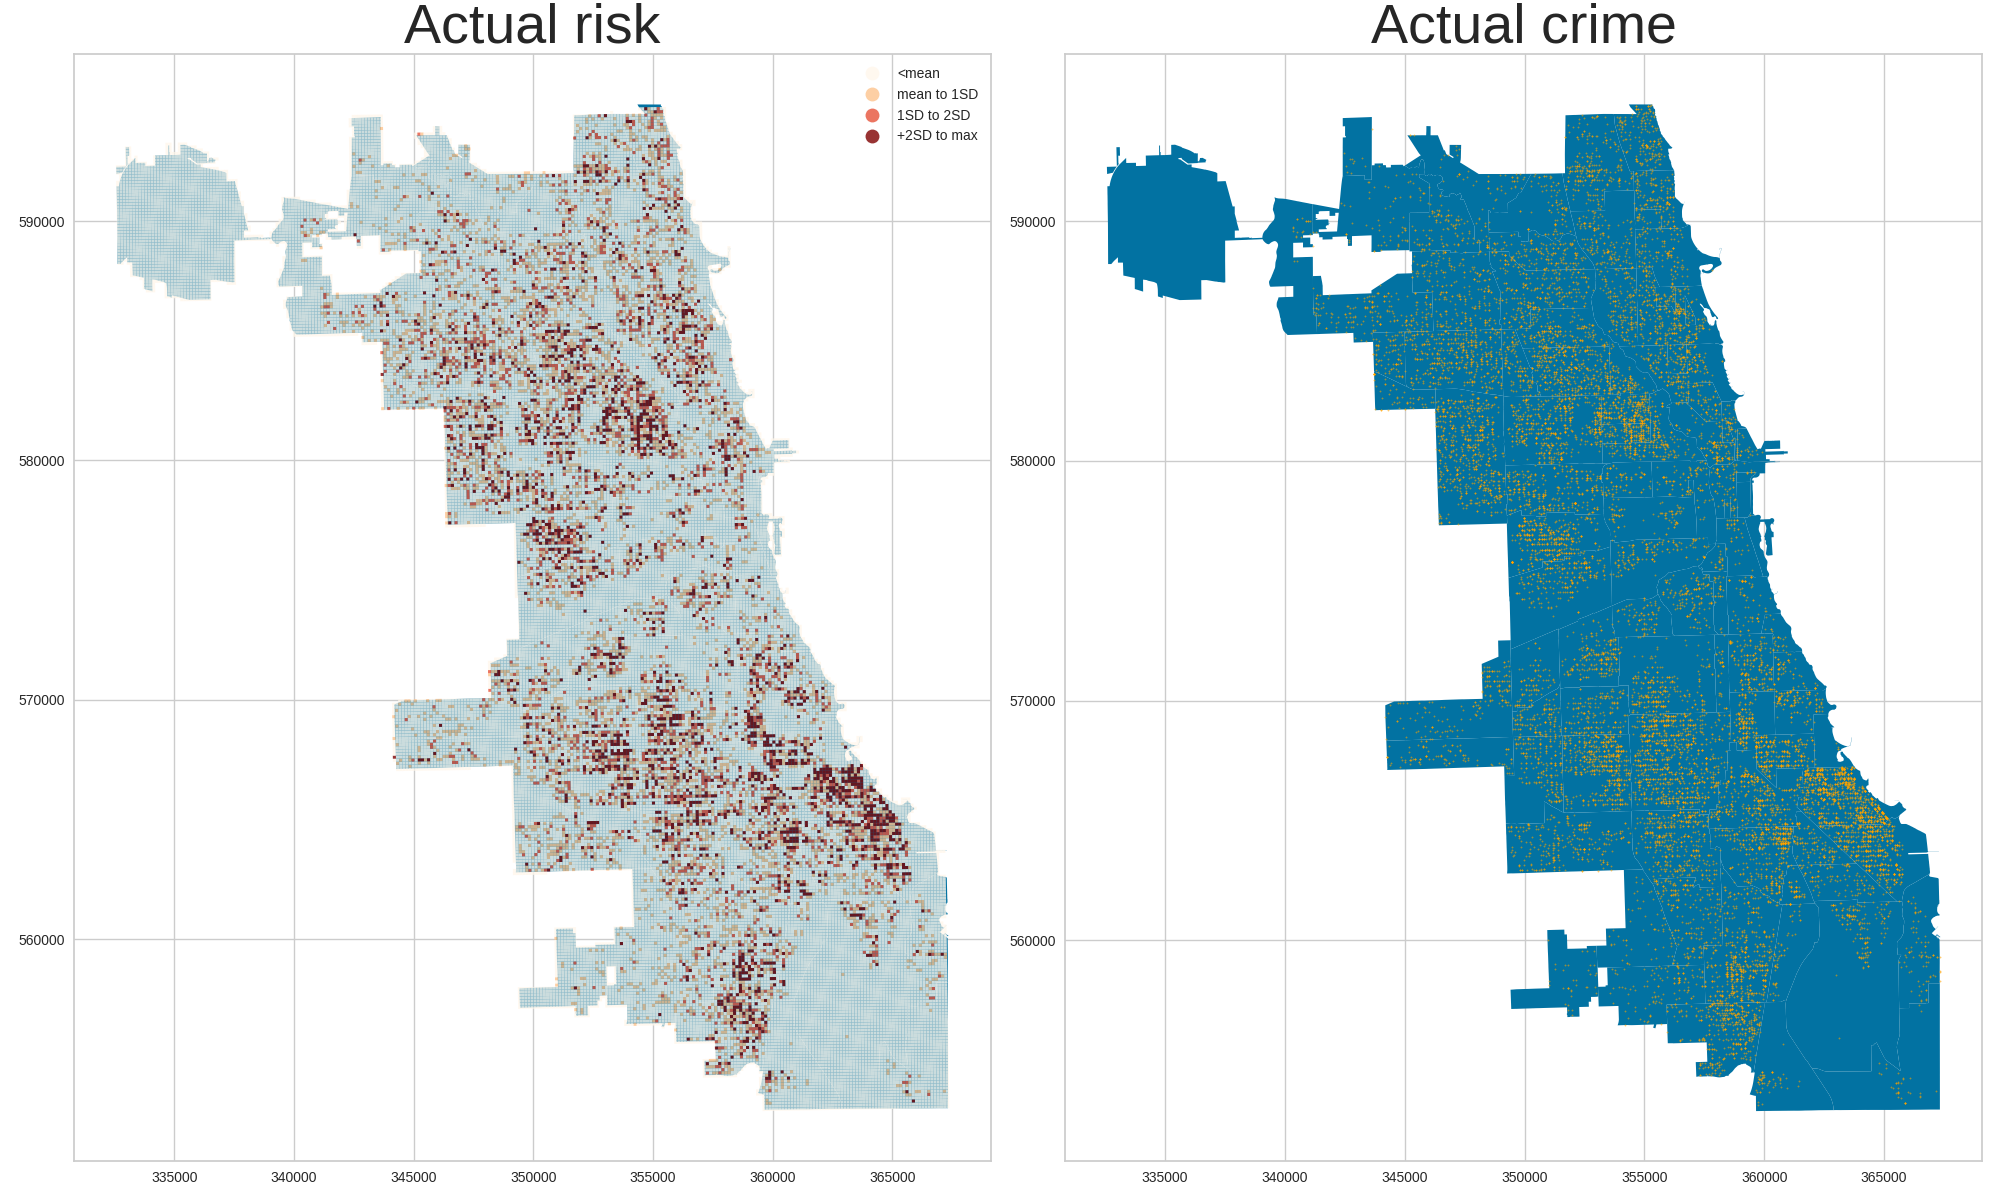
\includegraphics[scale=0.25]{./non-crime-val-figure/actual_risk_point_map.png}
  \caption{左:実際のリスクマップ 右:実際の強盗犯罪発生地点}
  \label{fig:nc-val-actual}
\end{figure}

\begin{figure}
  \centering % 図を中央寄せにする
  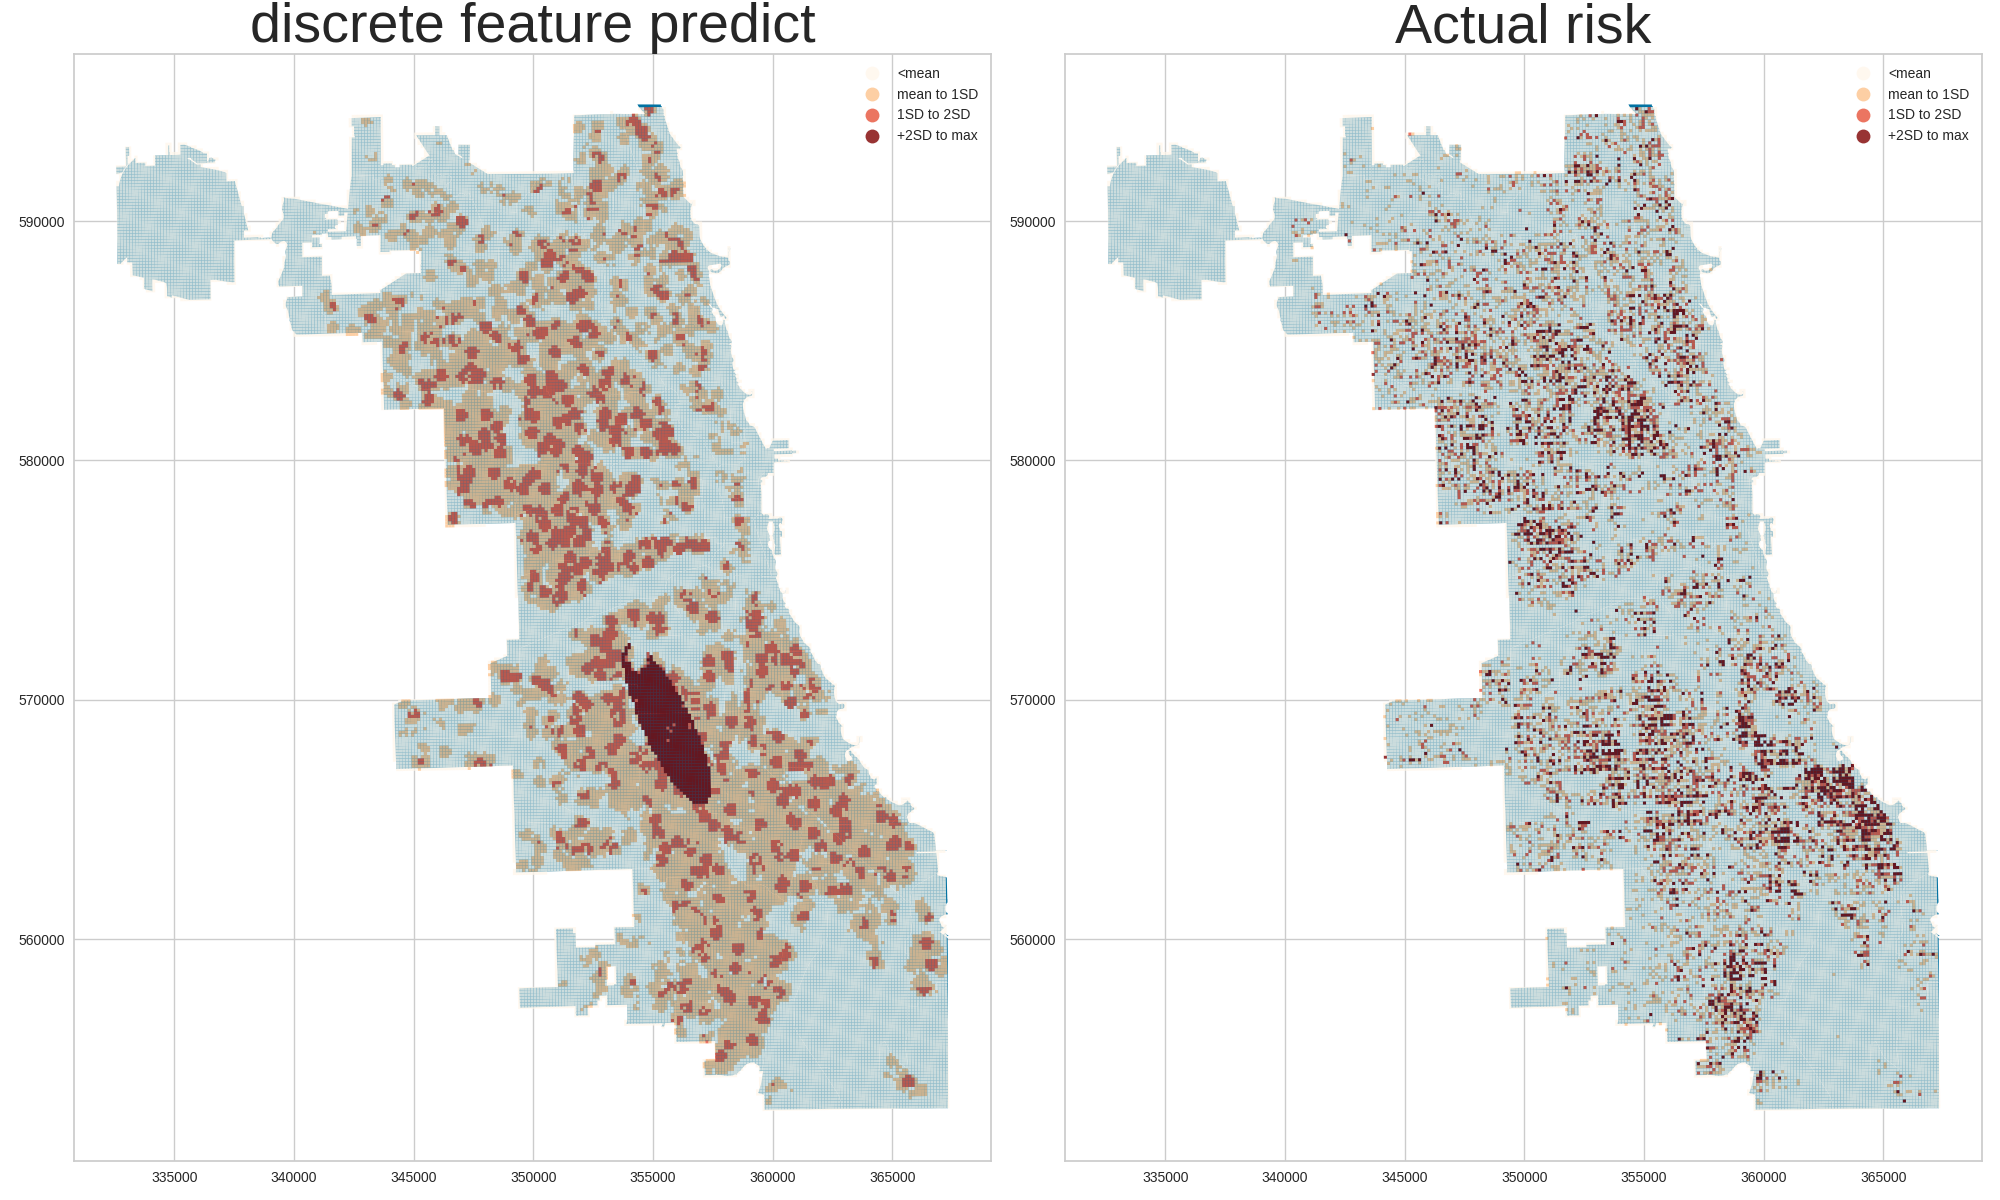
\includegraphics[scale=0.25]{./non-crime-val-figure/discrete_riskmap.png}
  \caption{左:離散型特徴量によるリスクマップ 右:実際のリスクマップ}
  \label{fig:nc-val-discrete}
\end{figure}

\begin{figure}
  \centering % 図を中央寄せにする
  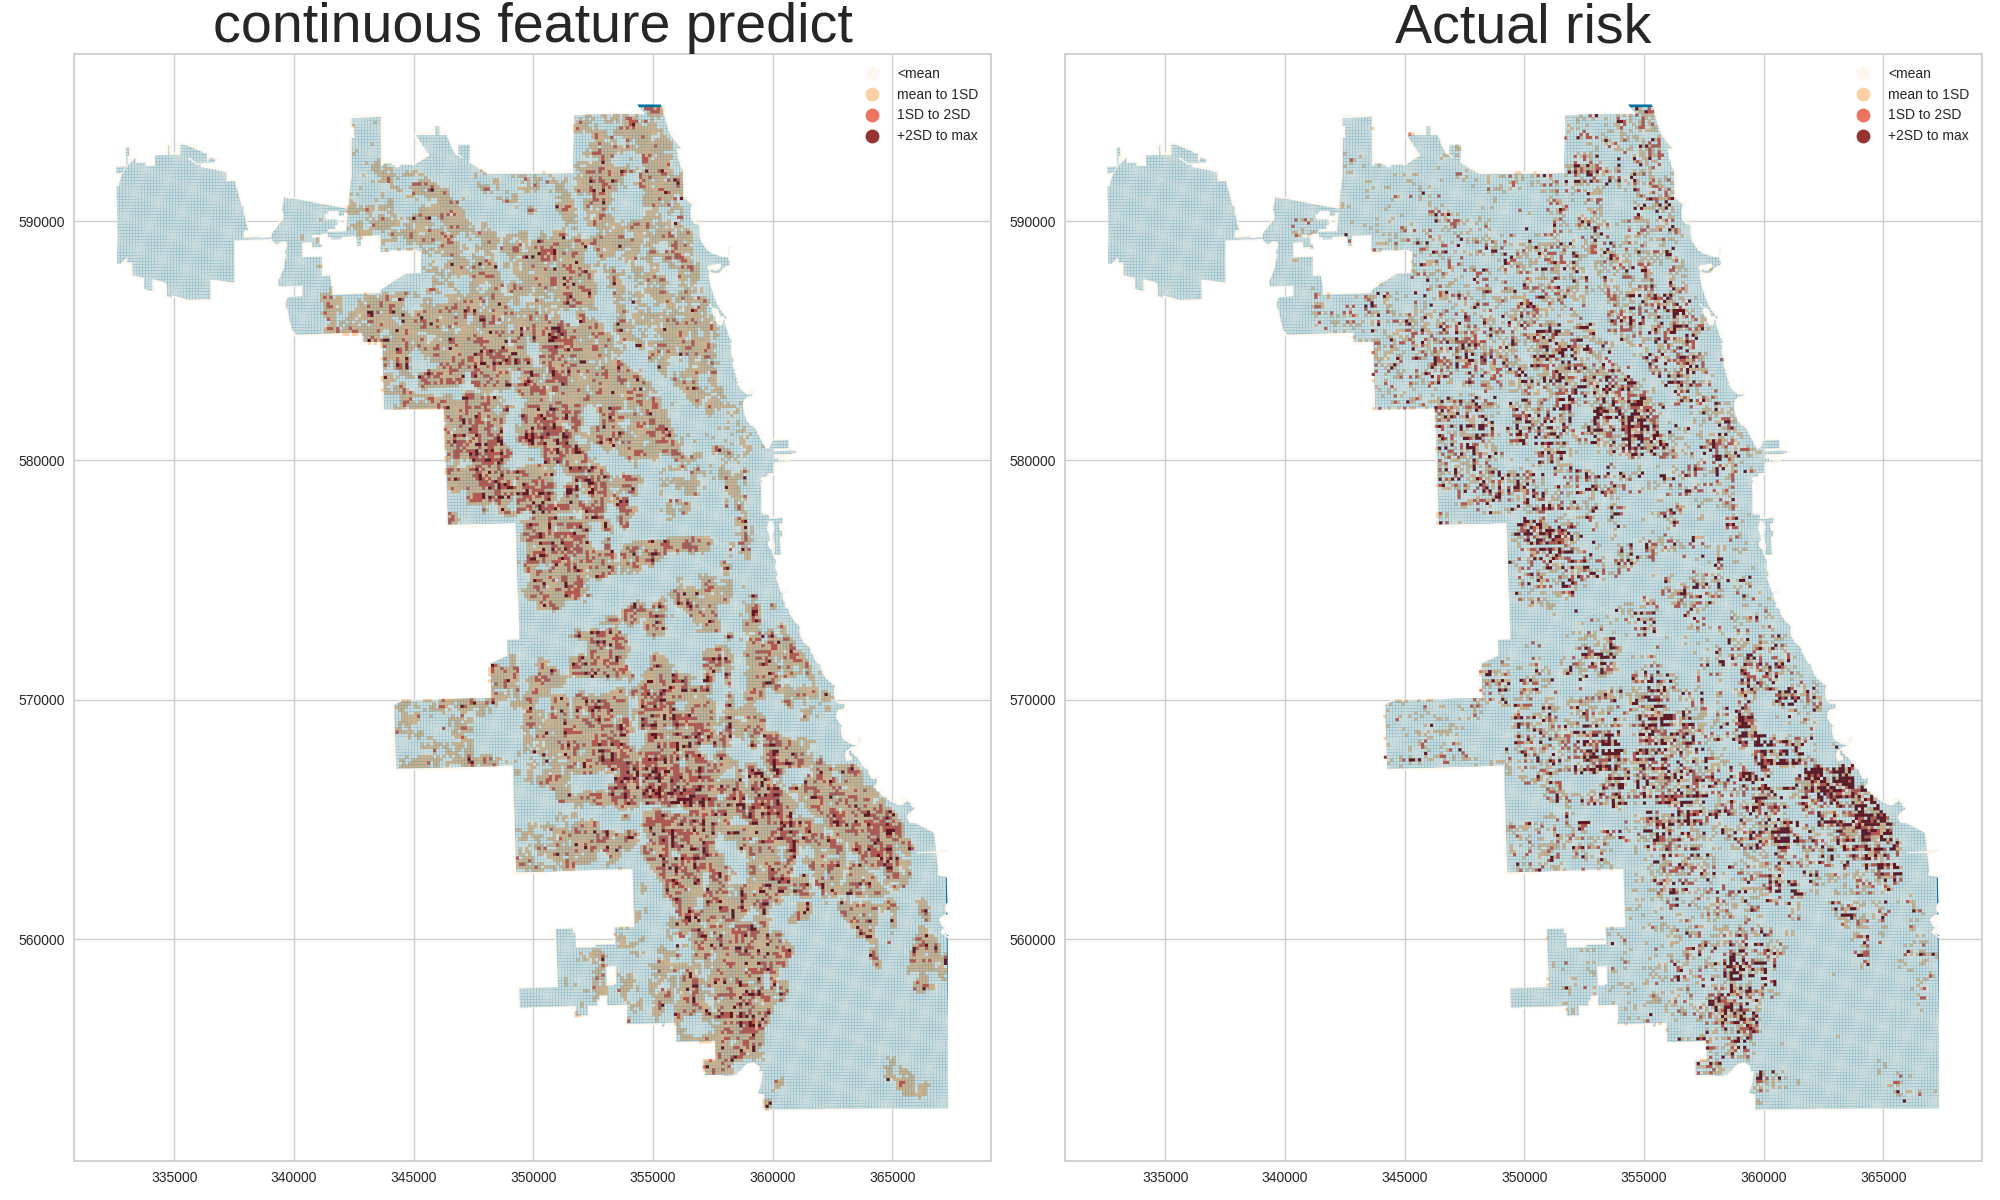
\includegraphics[scale=0.25]{./non-crime-val-figure/continuous_riskmap.png}
  \caption{左:連続型特徴量によるリスクマップ 右:実際のリスクマップ}
  \label{fig:nc-val-continuous}
\end{figure}

\begin{figure}
  \centering % 図を中央寄せにする
  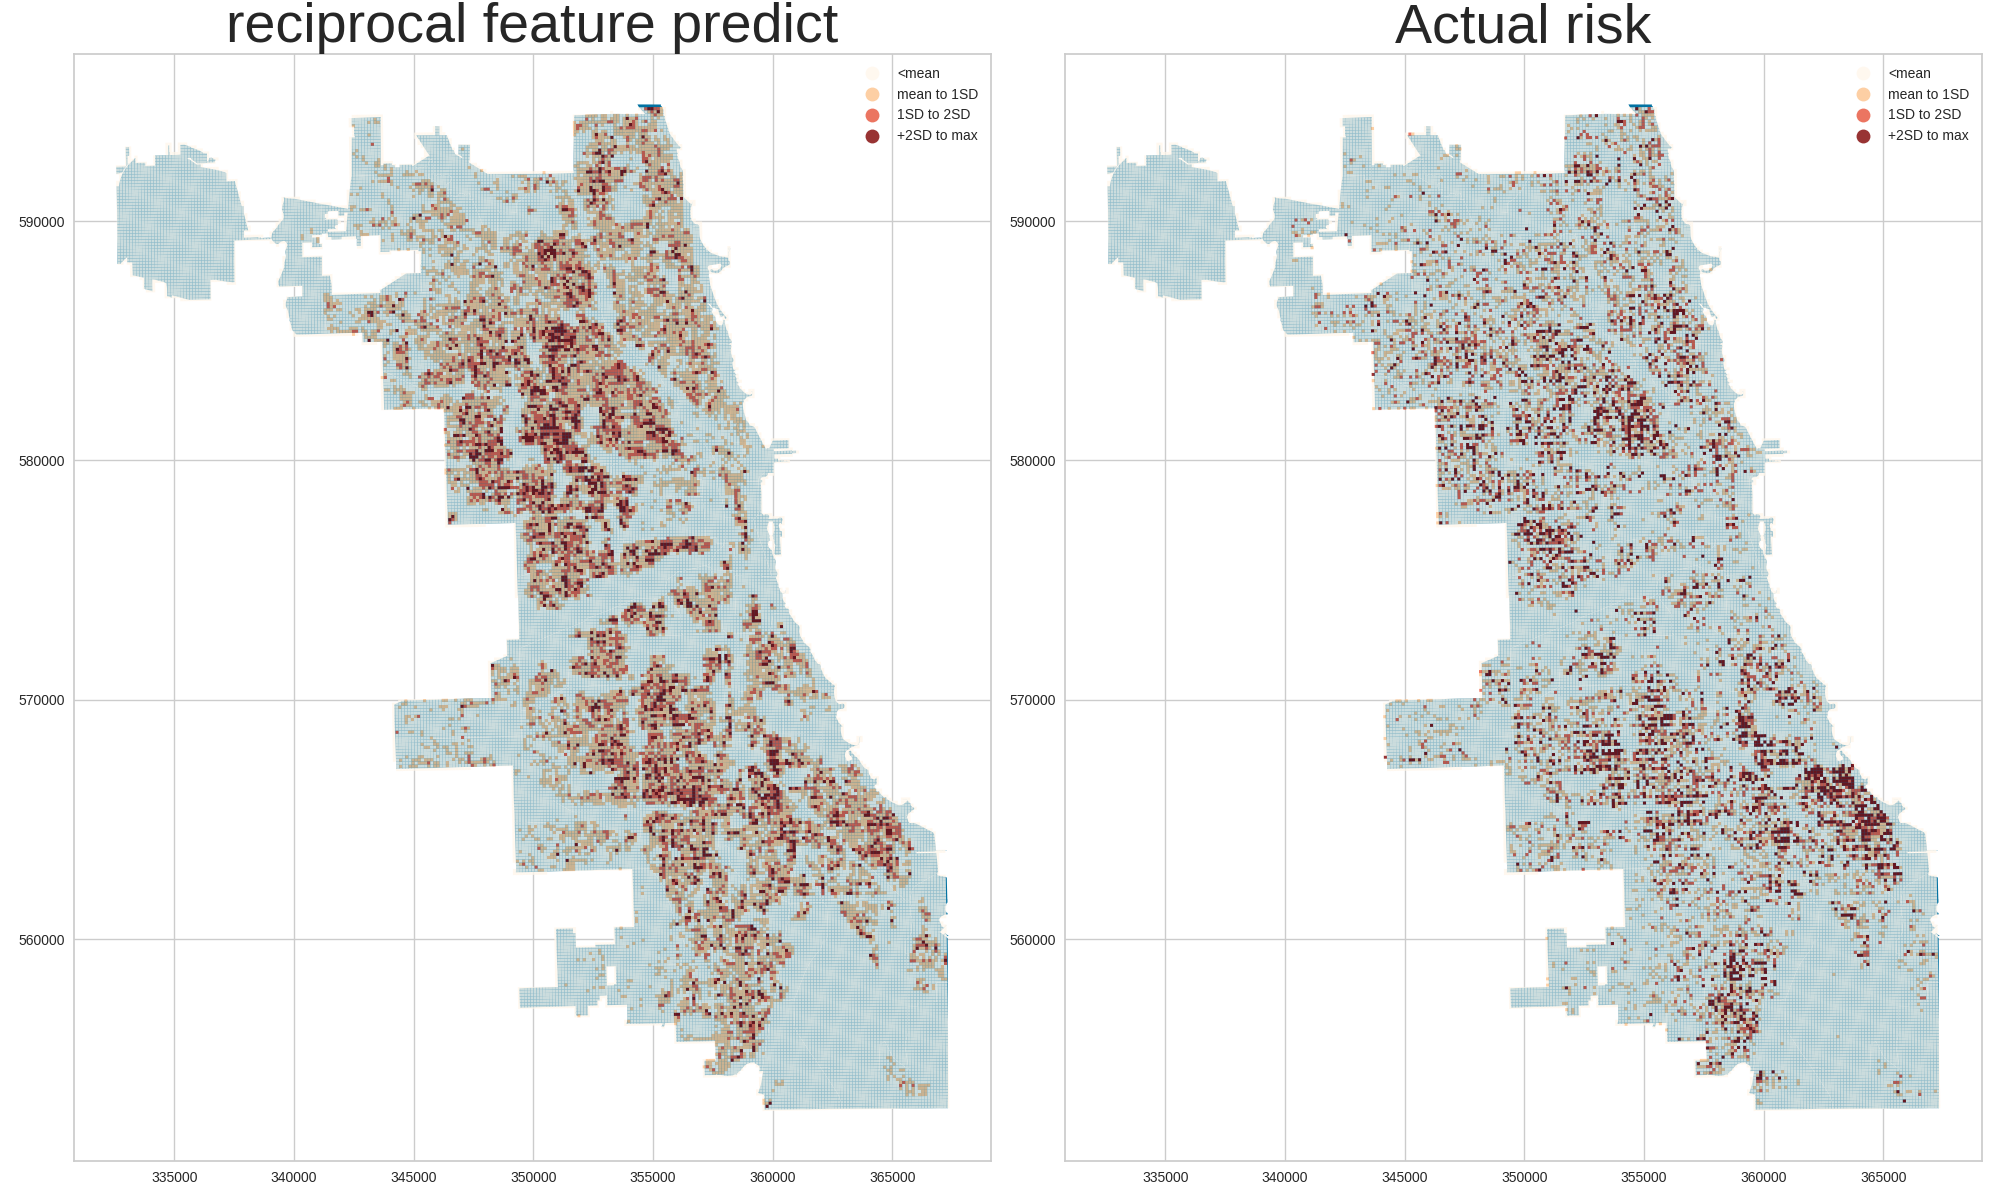
\includegraphics[scale=0.25]{./non-crime-val-figure/reciprocal_riskmap.png}
  \caption{左:逆数特徴量によるリスクマップ 右:実際のリスクマップ}
  \label{fig:nc-val-reciprocal}
\end{figure}

\begin{figure}
  \centering % 図を中央寄せにする
  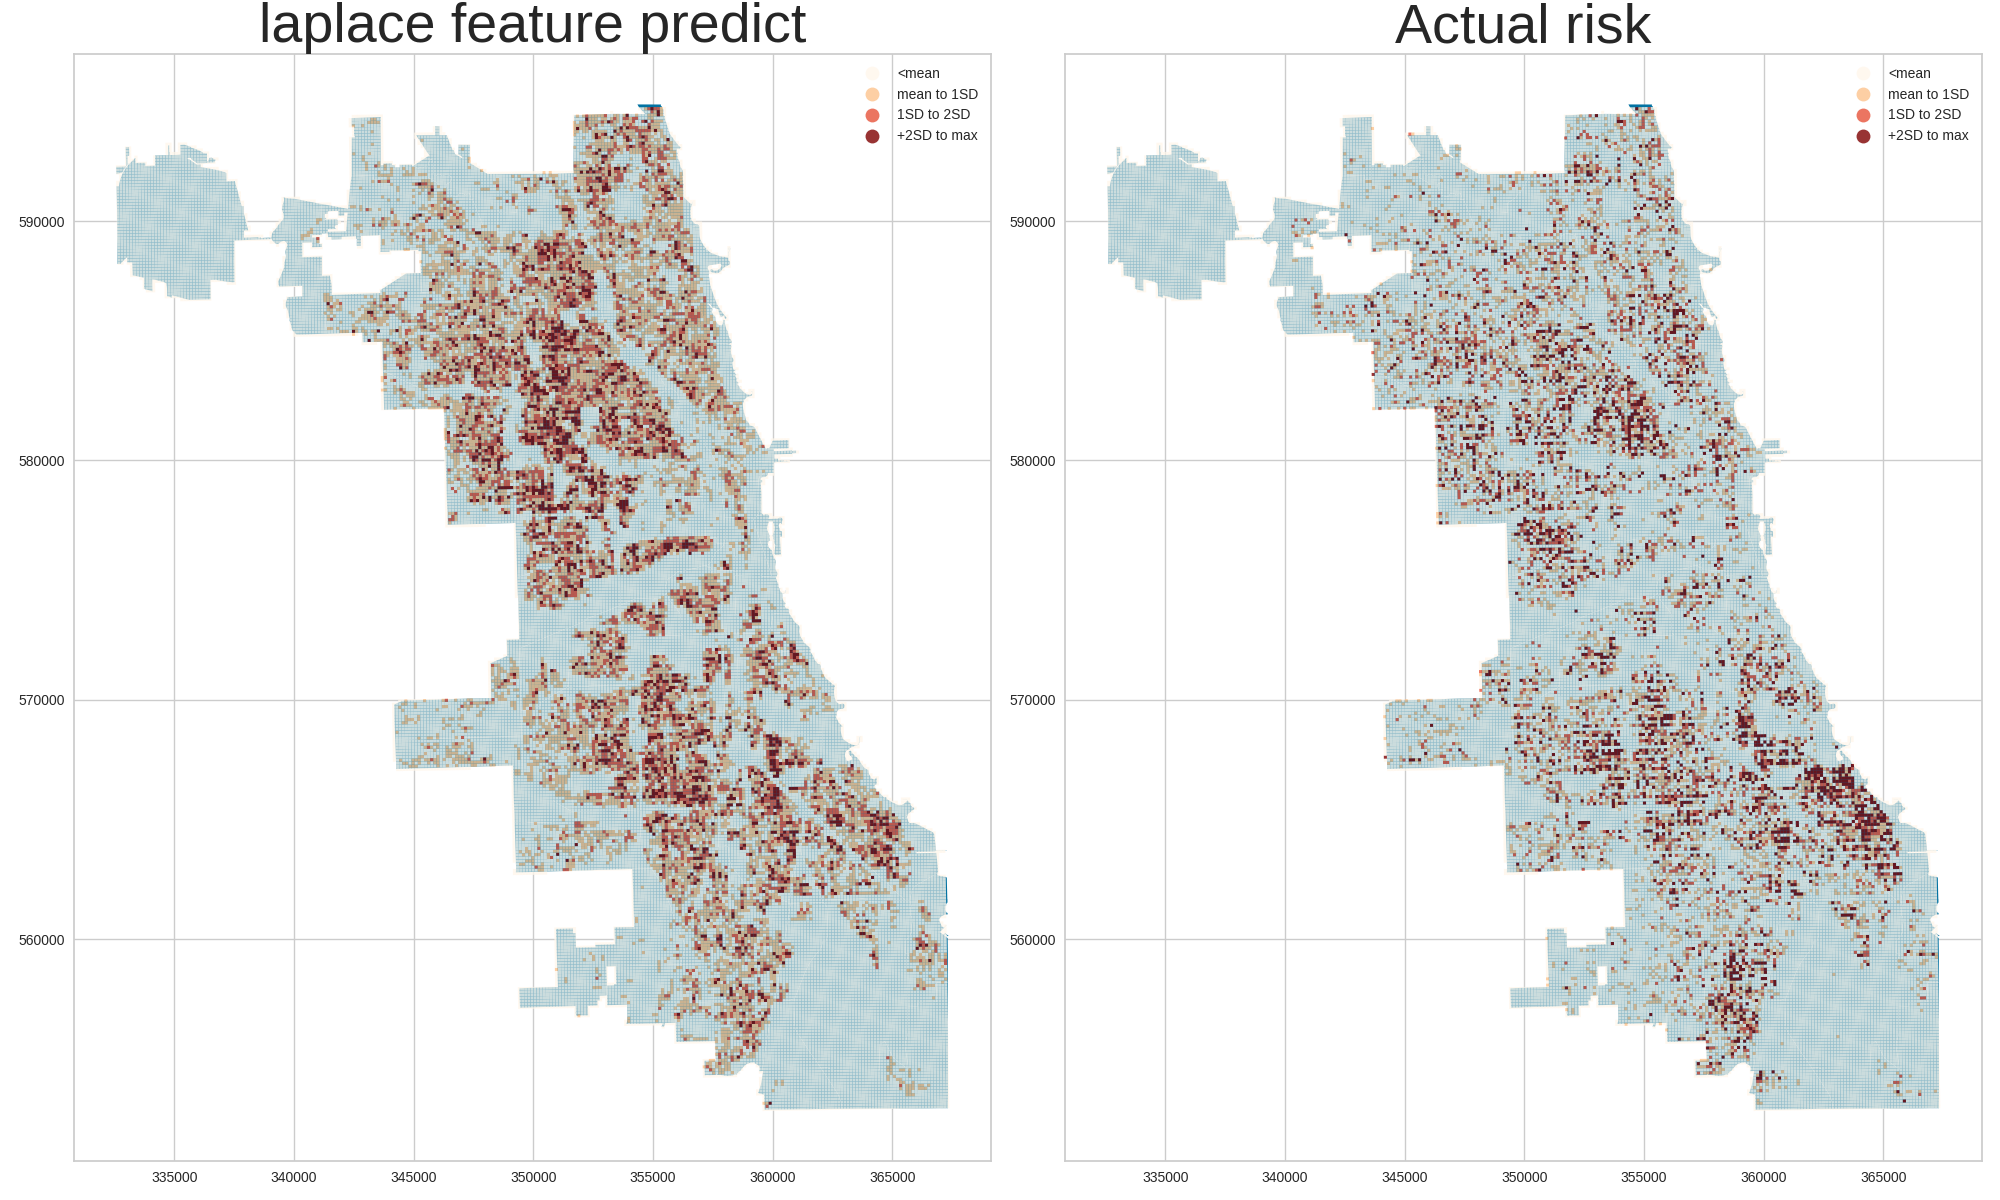
\includegraphics[scale=0.25]{./non-crime-val-figure/laplace_riskmap.png}
  \caption{左:ラプラス分布関数特徴量によるリスクマップ 右:実際のリスクマップ}
  \label{fig:nc-val-laplace}
\end{figure}

\begin{figure}
  \centering % 図を中央寄せにする
  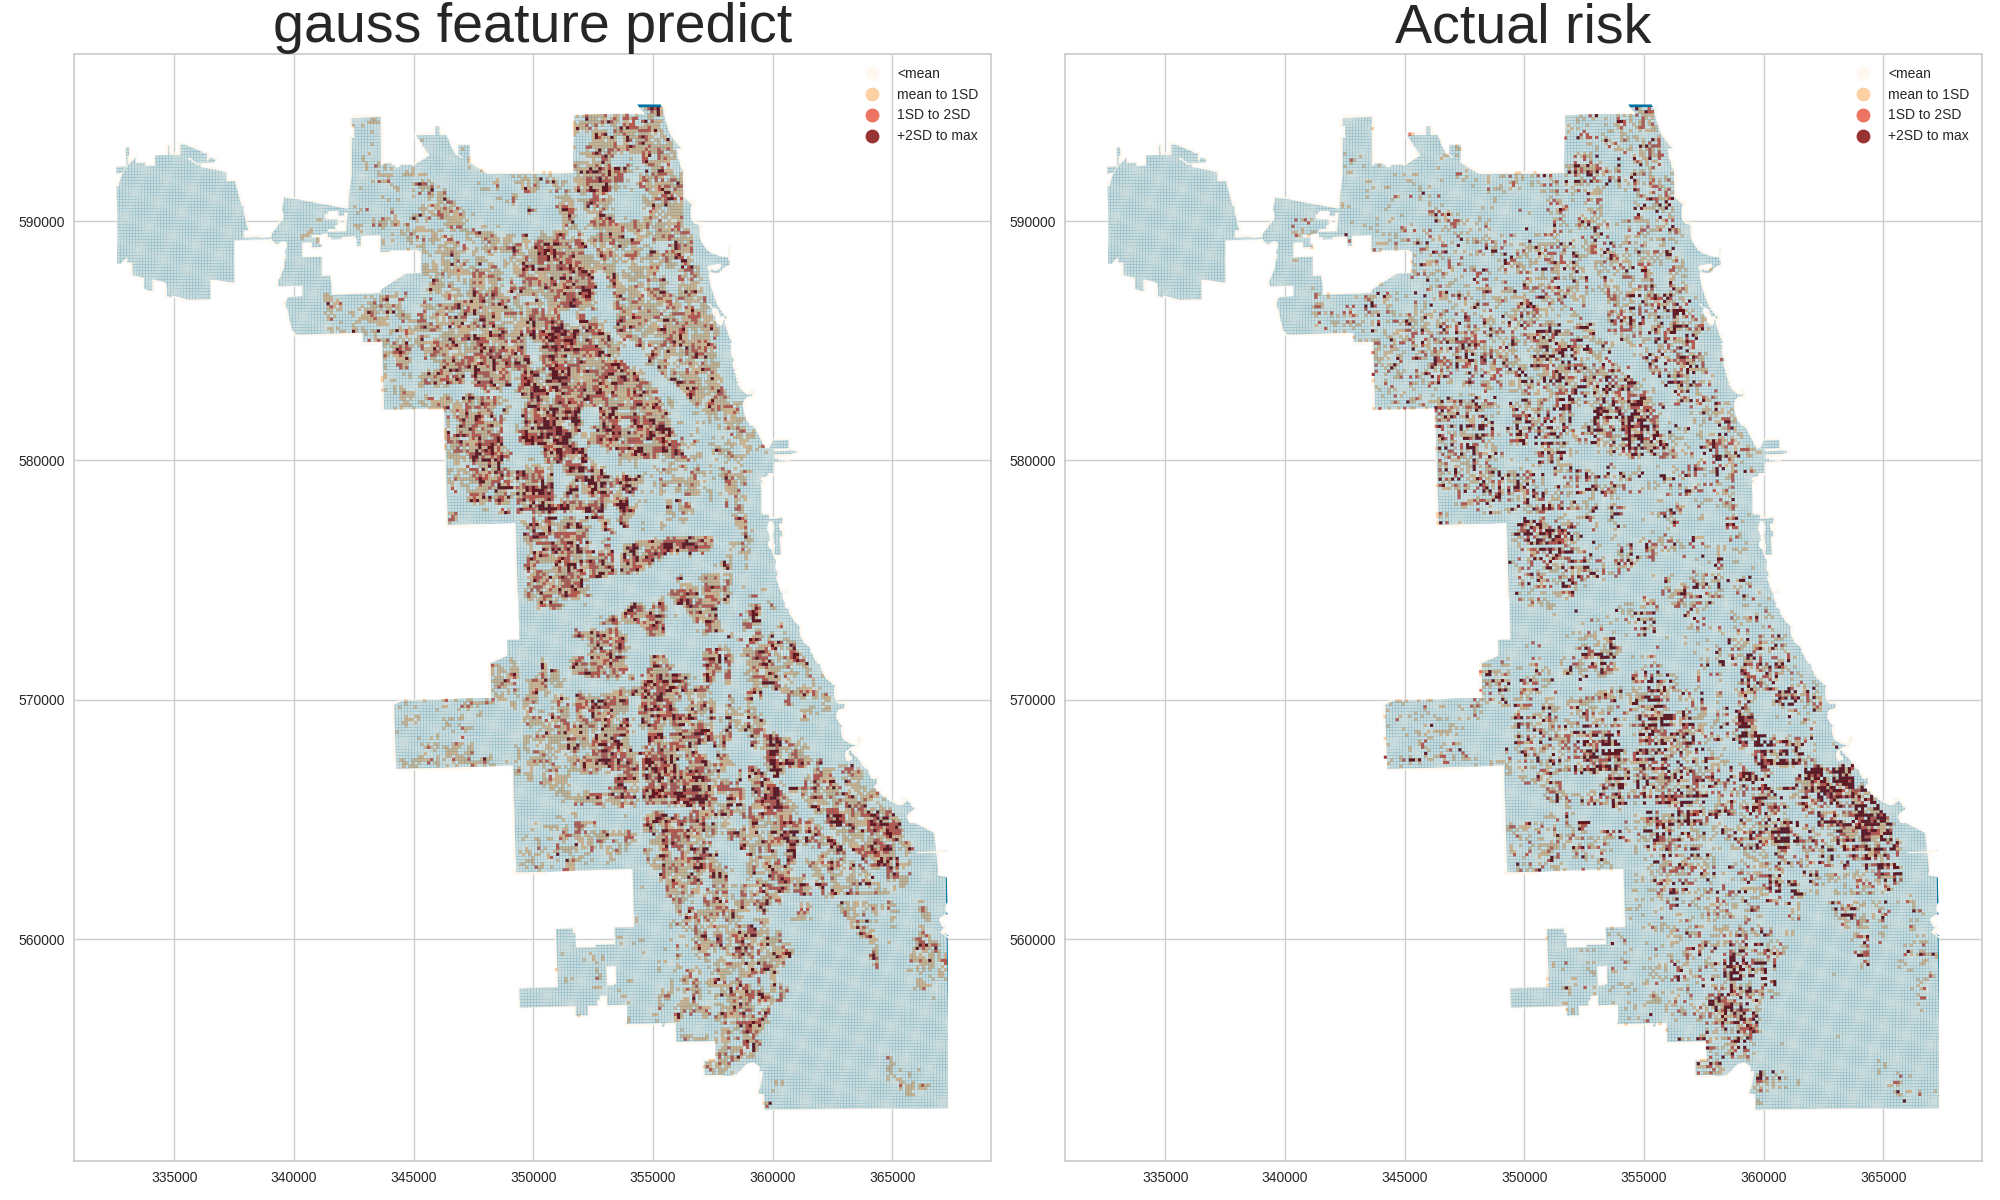
\includegraphics[scale=0.25]{./non-crime-val-figure/gauss_riskmap.png}
  \caption{左:ガウス関数特徴量によるリスクマップ 右:実際のリスクマップ}
  \label{fig:nc-val-gauss}
\end{figure}

各モデルの予測値を4カテゴリーに分割した混同行列をに示す.
各モデルの予測値を4カテゴリーに分割した混同行列をに示す.
\begin{figure}
  \centering % 図を中央寄せにする
  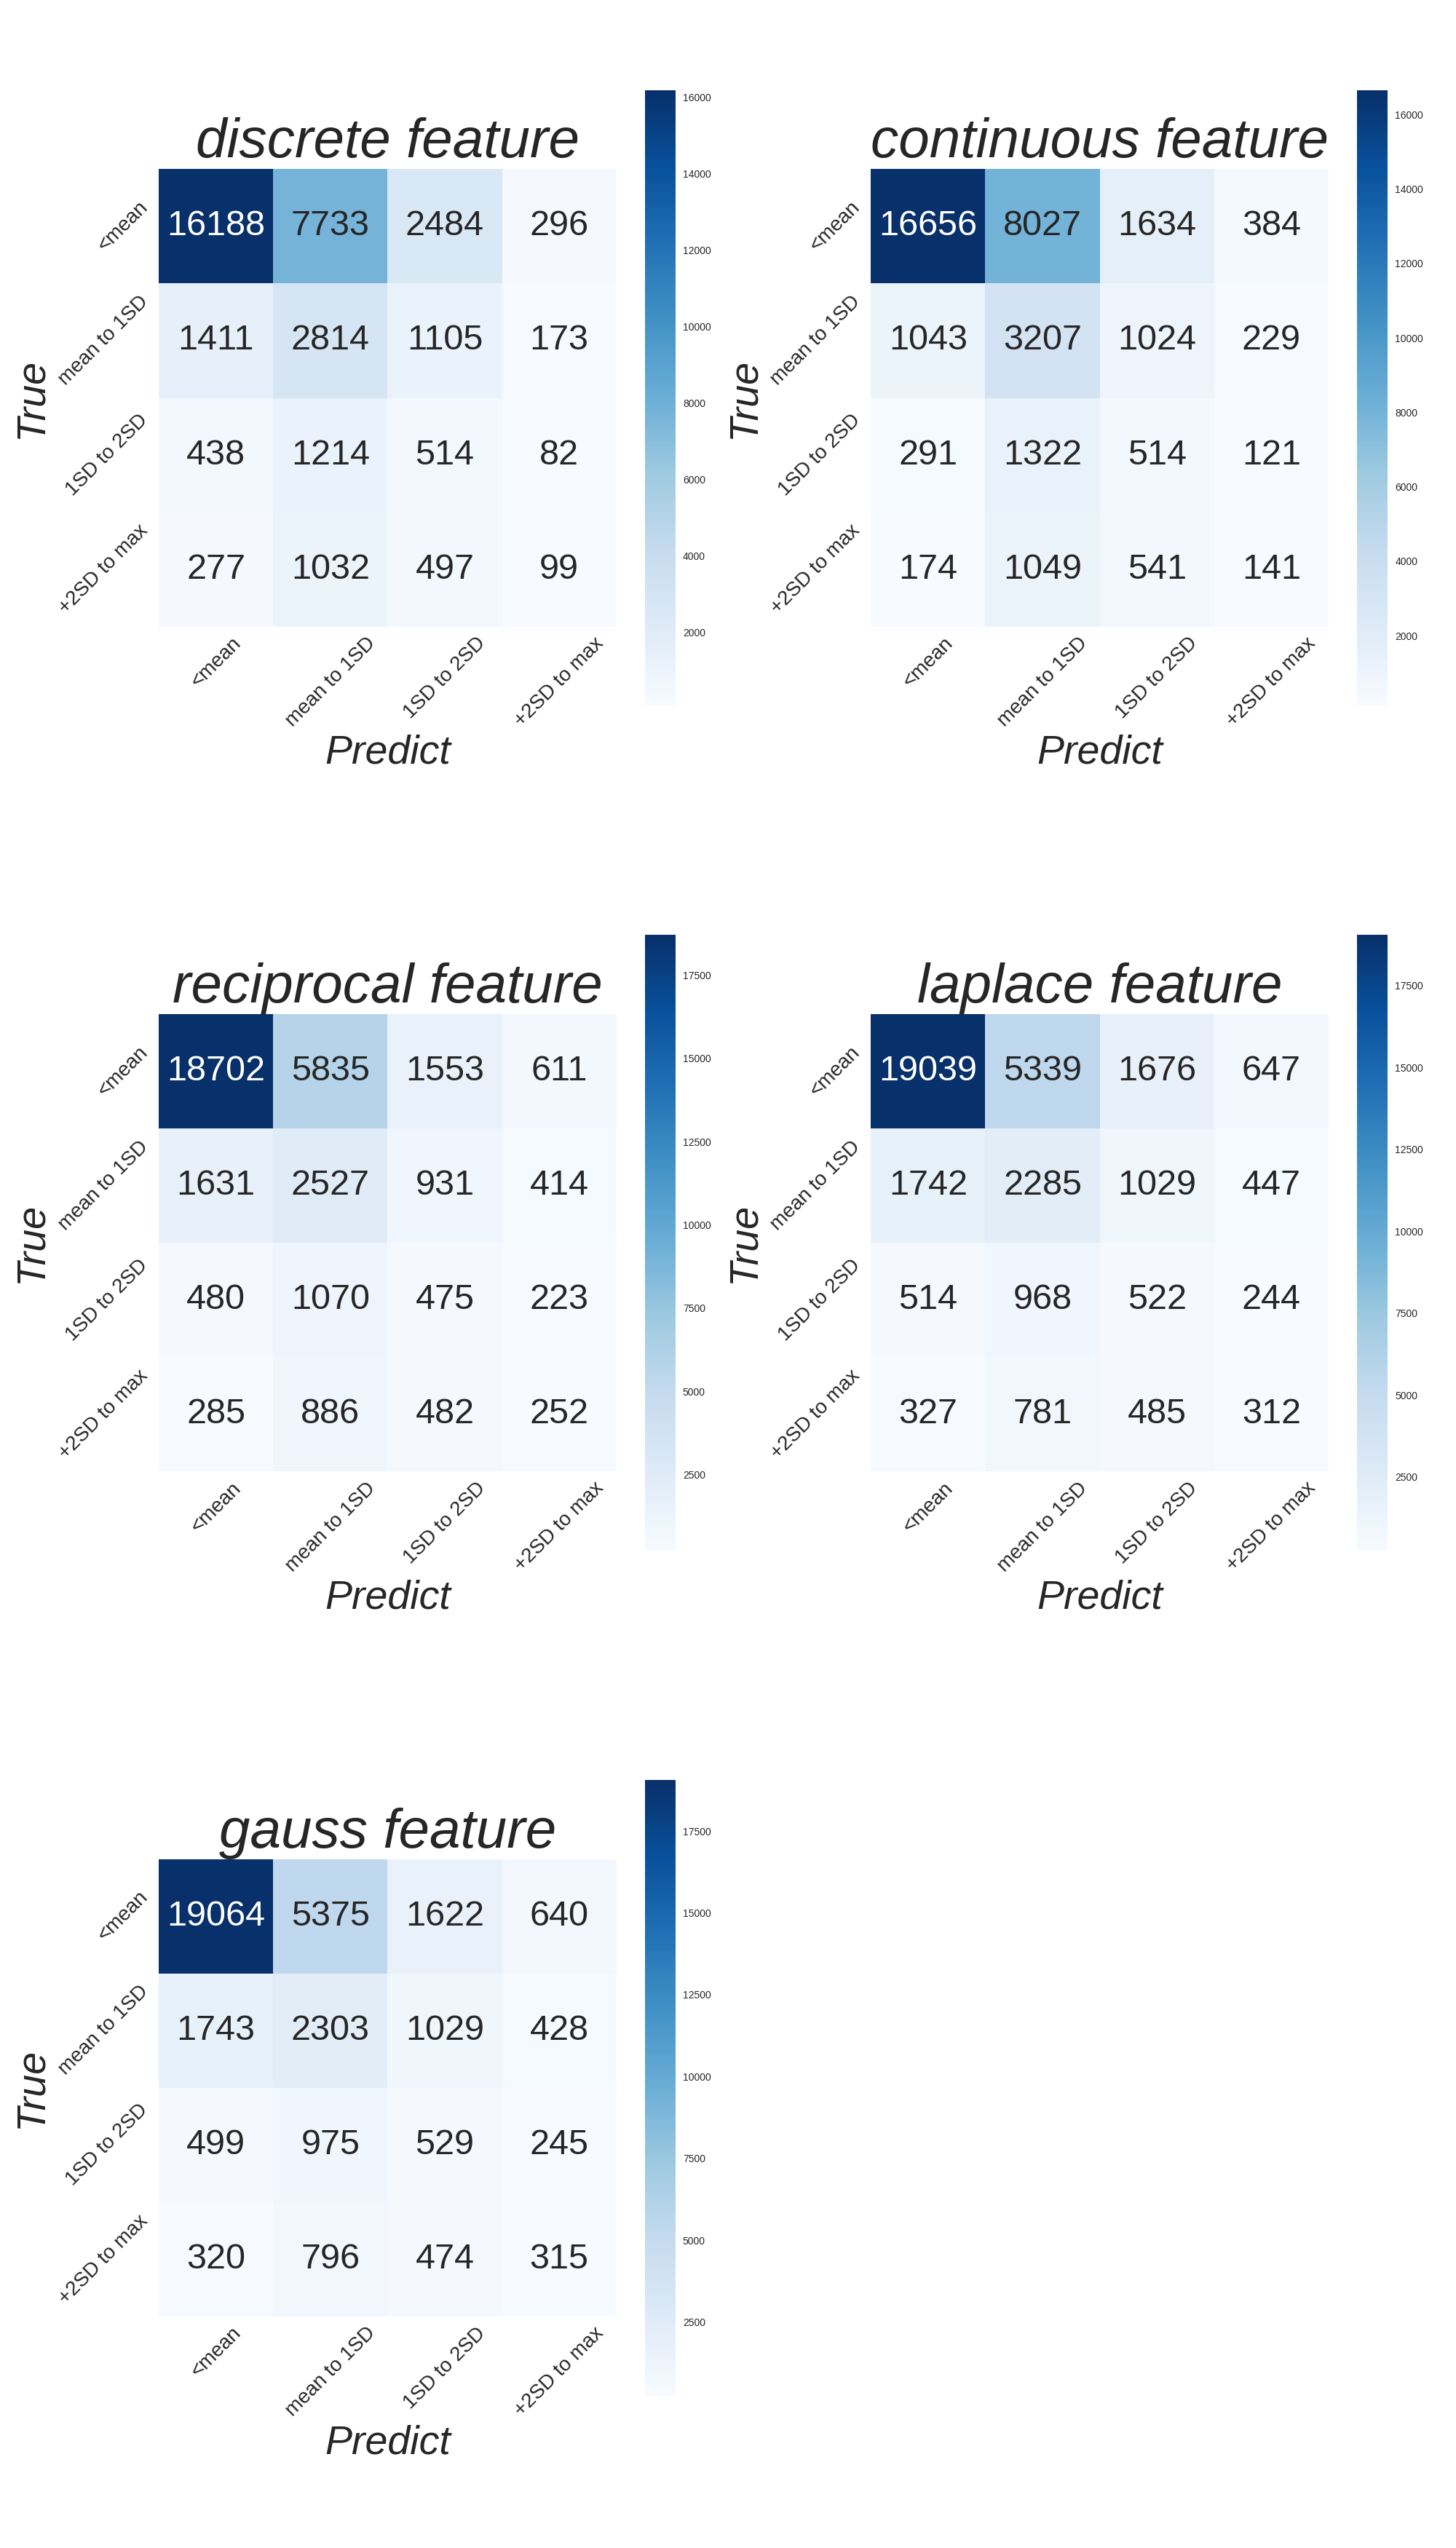
\includegraphics[scale=0.23]{./non-crime-val-figure/non_crime_val_four_cm.png}
  \caption{4カテゴリーの混同行列}
  \label{fig:nc-val-4cm}
\end{figure}

\begin{figure}
  \centering % 図を中央寄せにする
  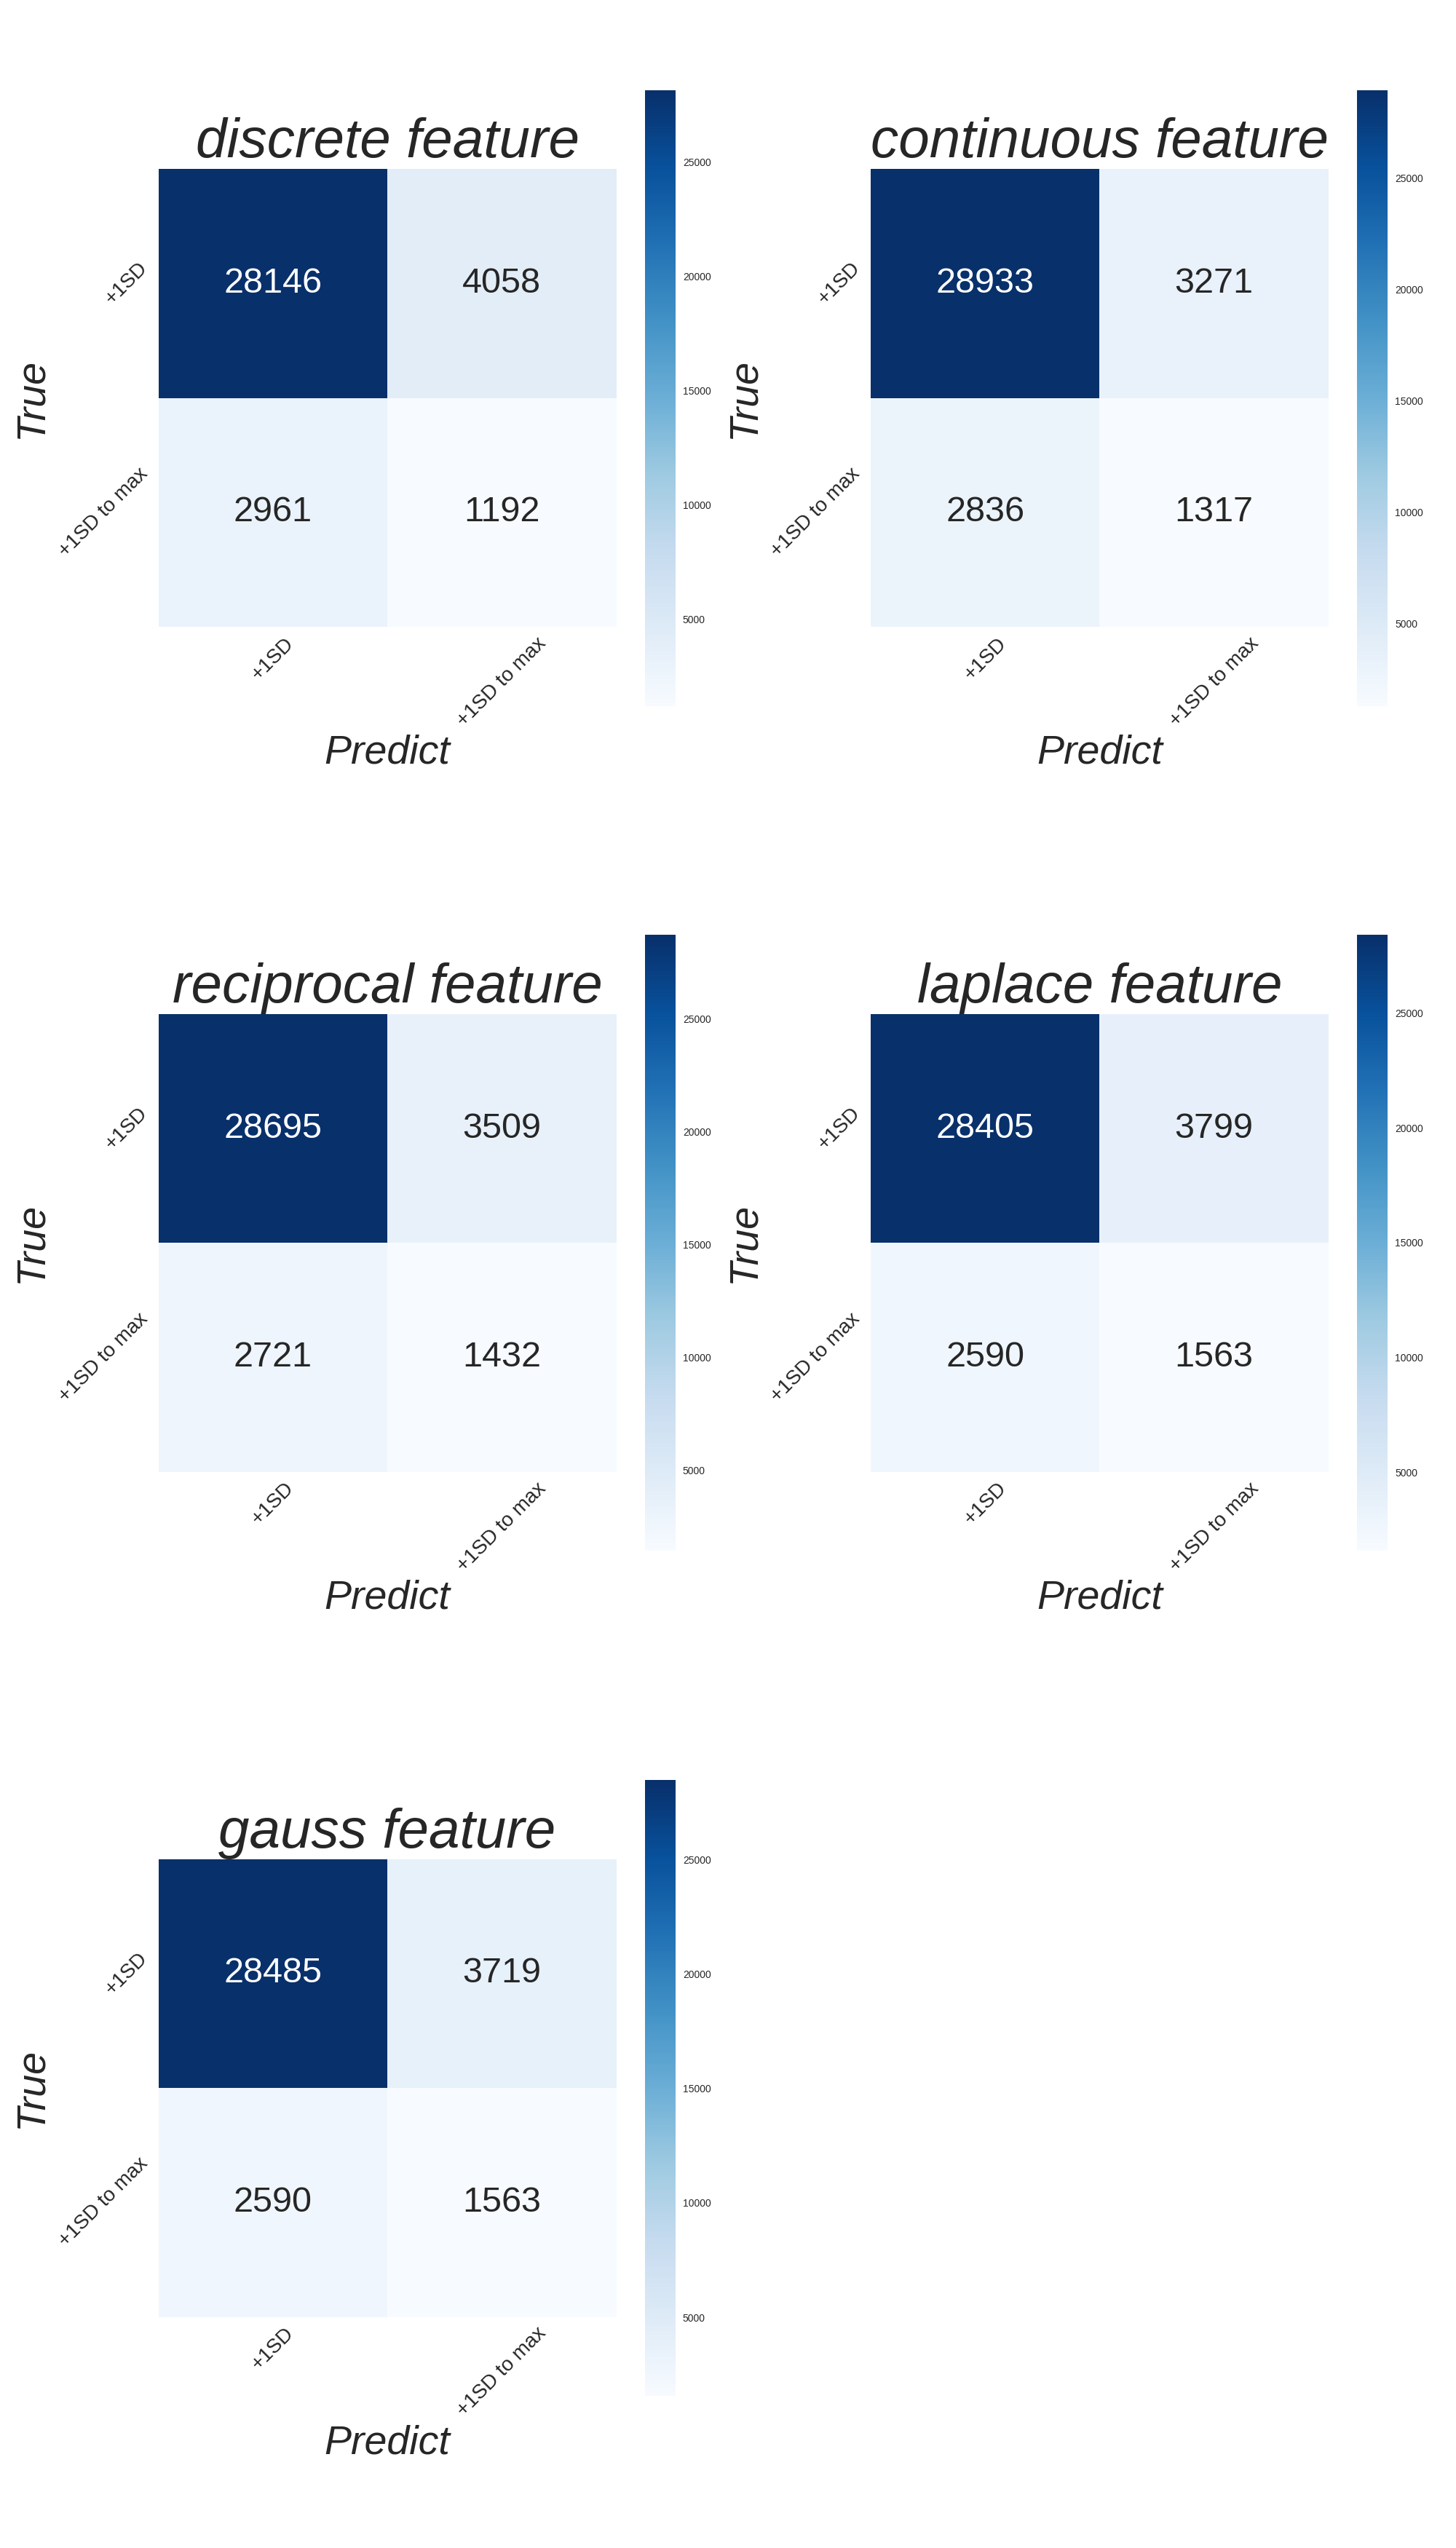
\includegraphics[scale=0.23]{./non-crime-val-figure/non_crime_val_two_cm.png}
  \caption{2カテゴリーの混同行列}
  \label{fig:nc-val-2cm}
\end{figure}
% ---------------------------------
% FNFPplot
% ---------------------------------
\begin{figure}
  \centering % 図を中央寄せにする
  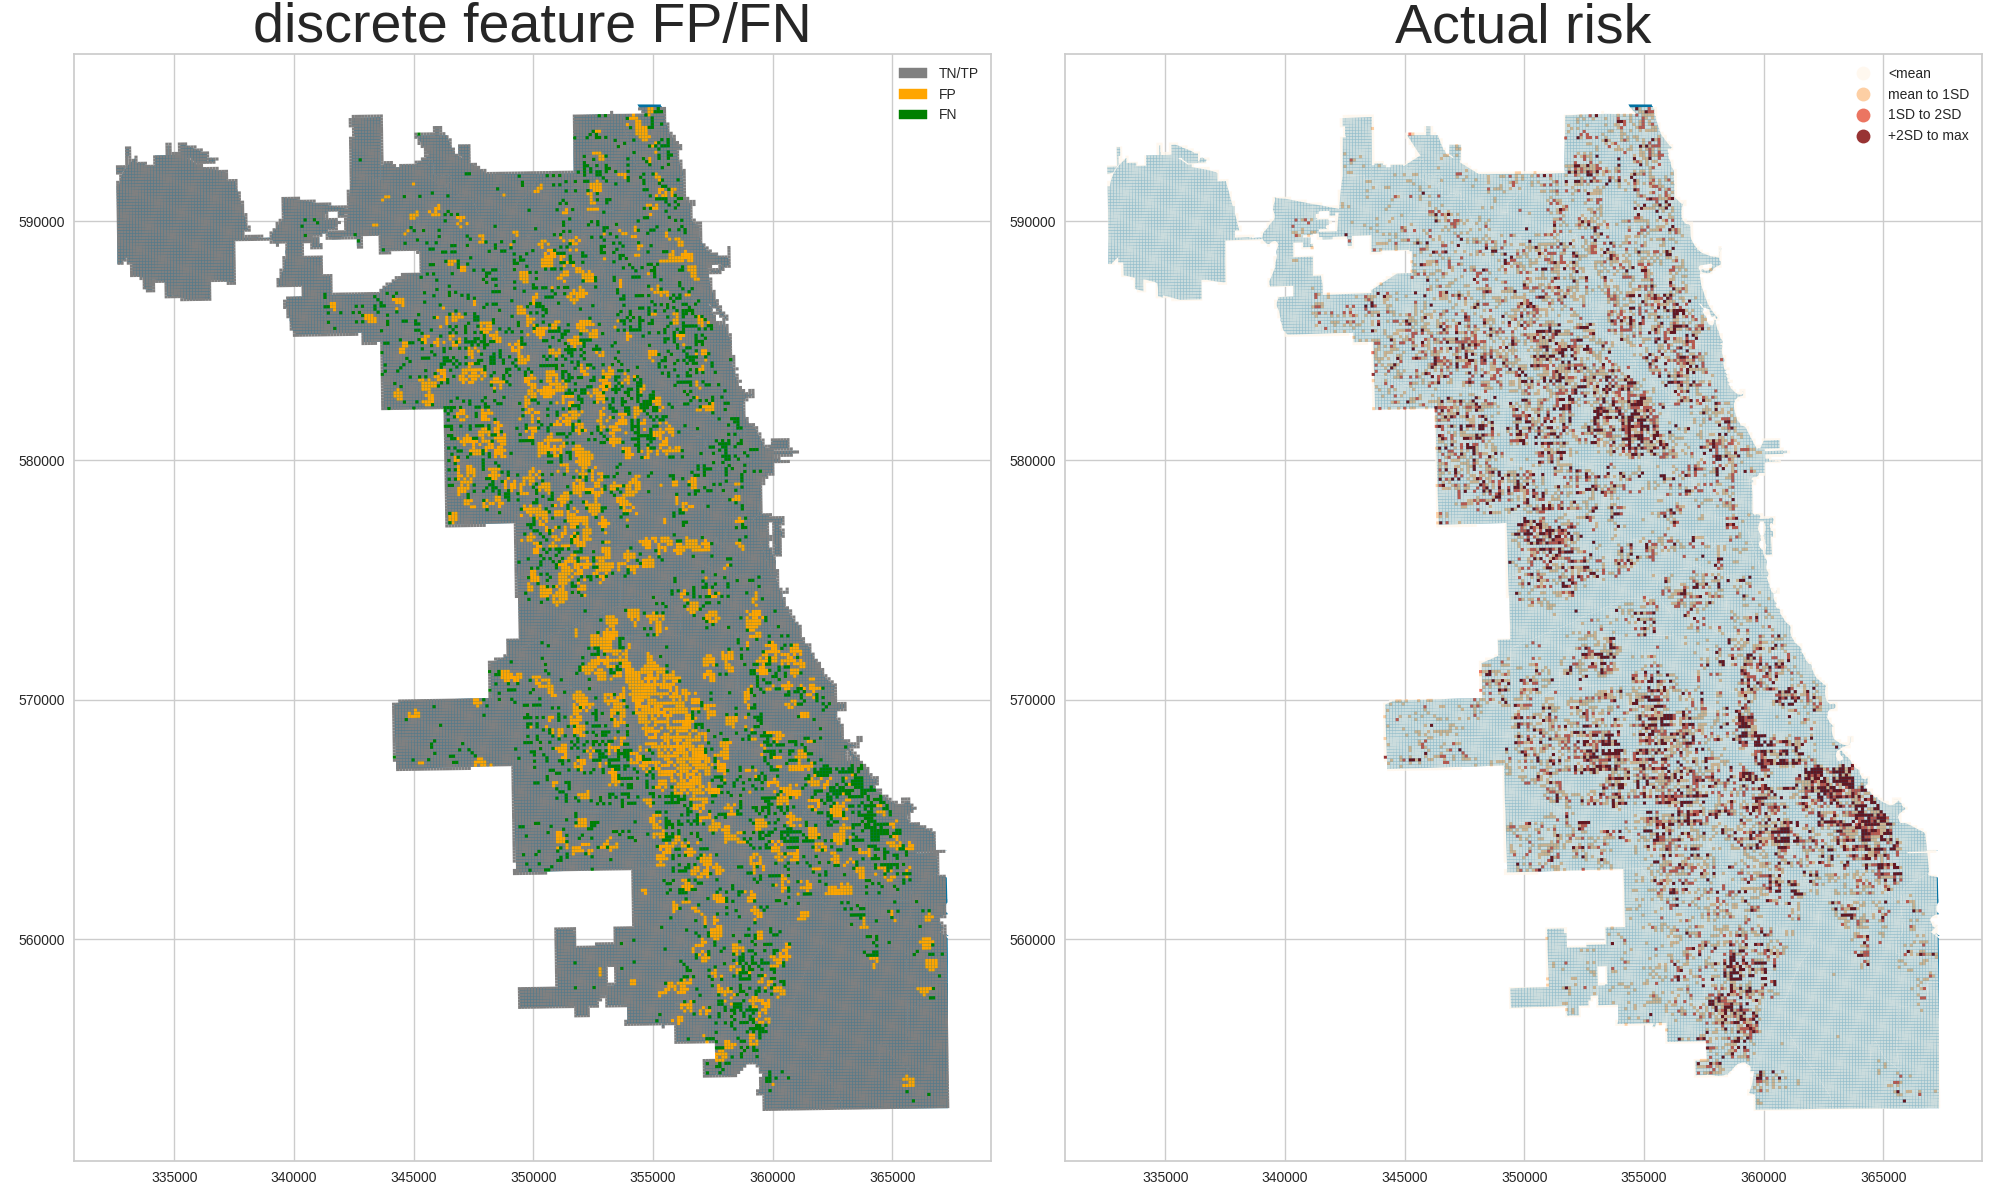
\includegraphics[scale=0.25]{./non-crime-val-figure/discrete_fnp.png}
  \caption{左:離散型特徴量のFPFN 右:実際のリスクマップ}
  \label{fig:nc-val-discrete-fnp}
\end{figure}

\begin{figure}
  \centering % 図を中央寄せにする
  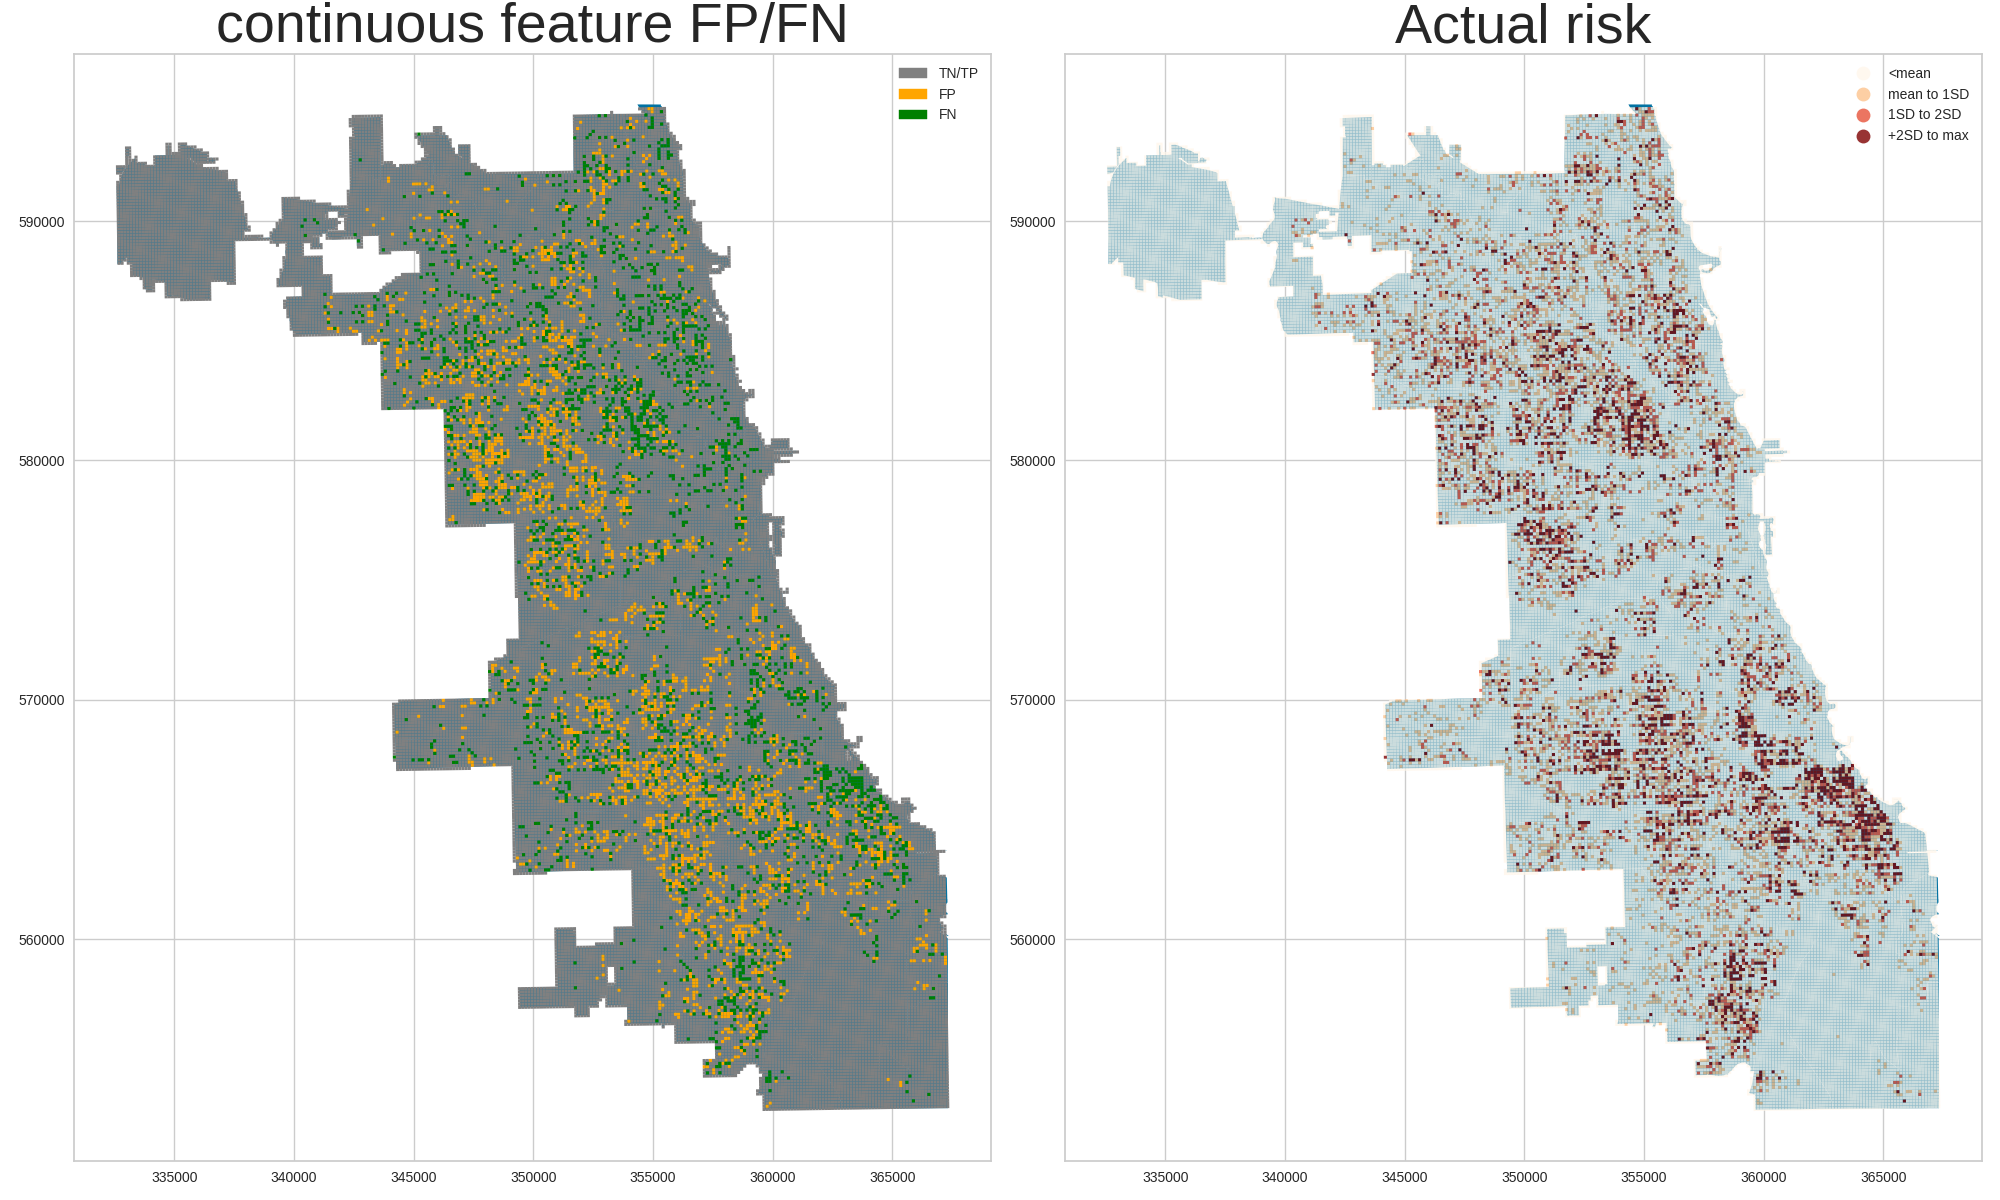
\includegraphics[scale=0.25]{./non-crime-val-figure/continuous_fnp.png}
  \caption{左:連続型特徴量のFPFN 右:実際のリスクマップ}
  \label{fig:nc-val-continuous-fnp}
\end{figure}

\begin{figure}
  \centering % 図を中央寄せにする
  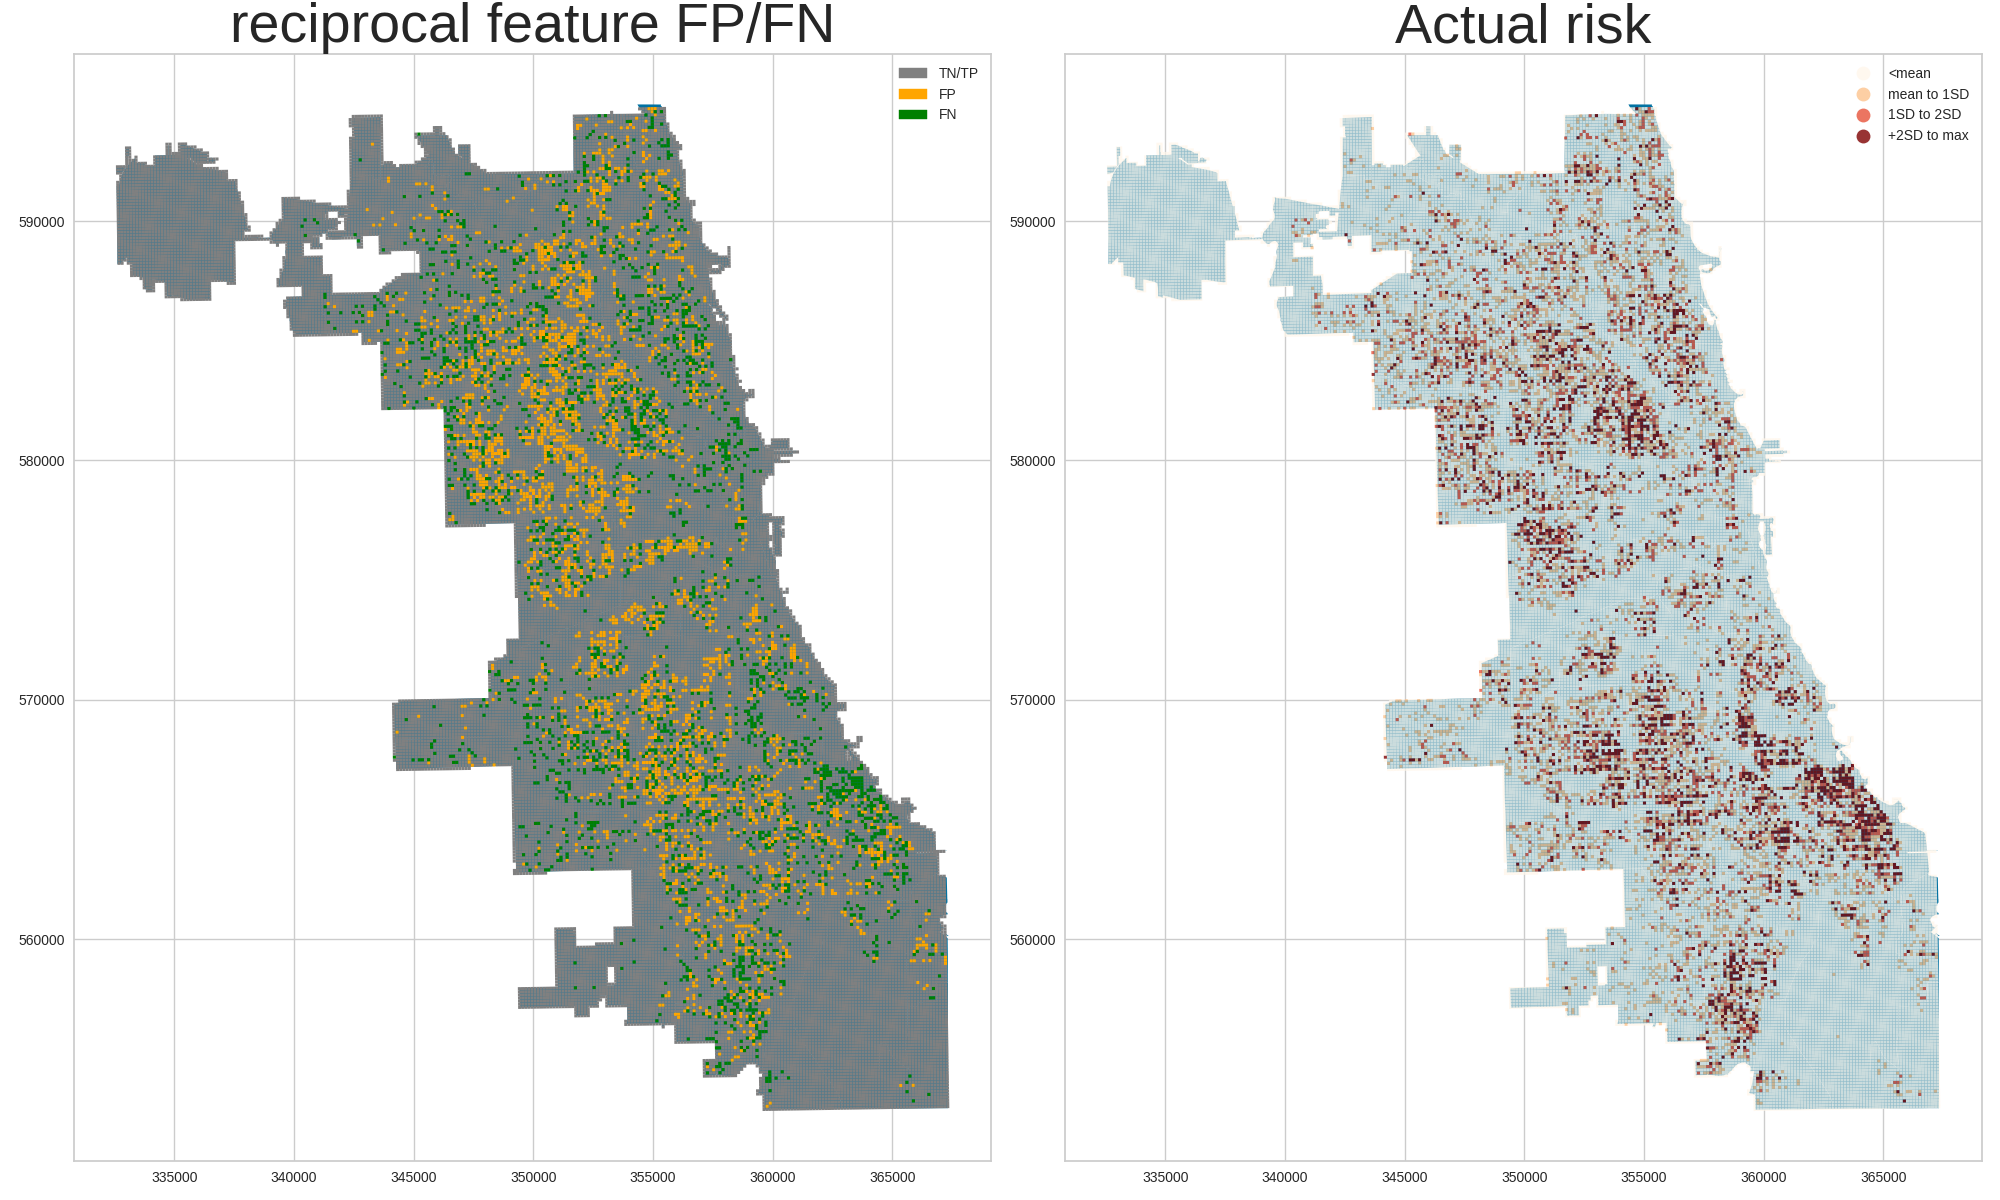
\includegraphics[scale=0.25]{./non-crime-val-figure/reciprocal_fnp.png}
  \caption{左:逆数特徴量のFPFN 右:実際のリスクマップ}
  \label{fig:nc-val-reciprocal-fnp}
\end{figure}

\begin{figure}
  \centering % 図を中央寄せにする
  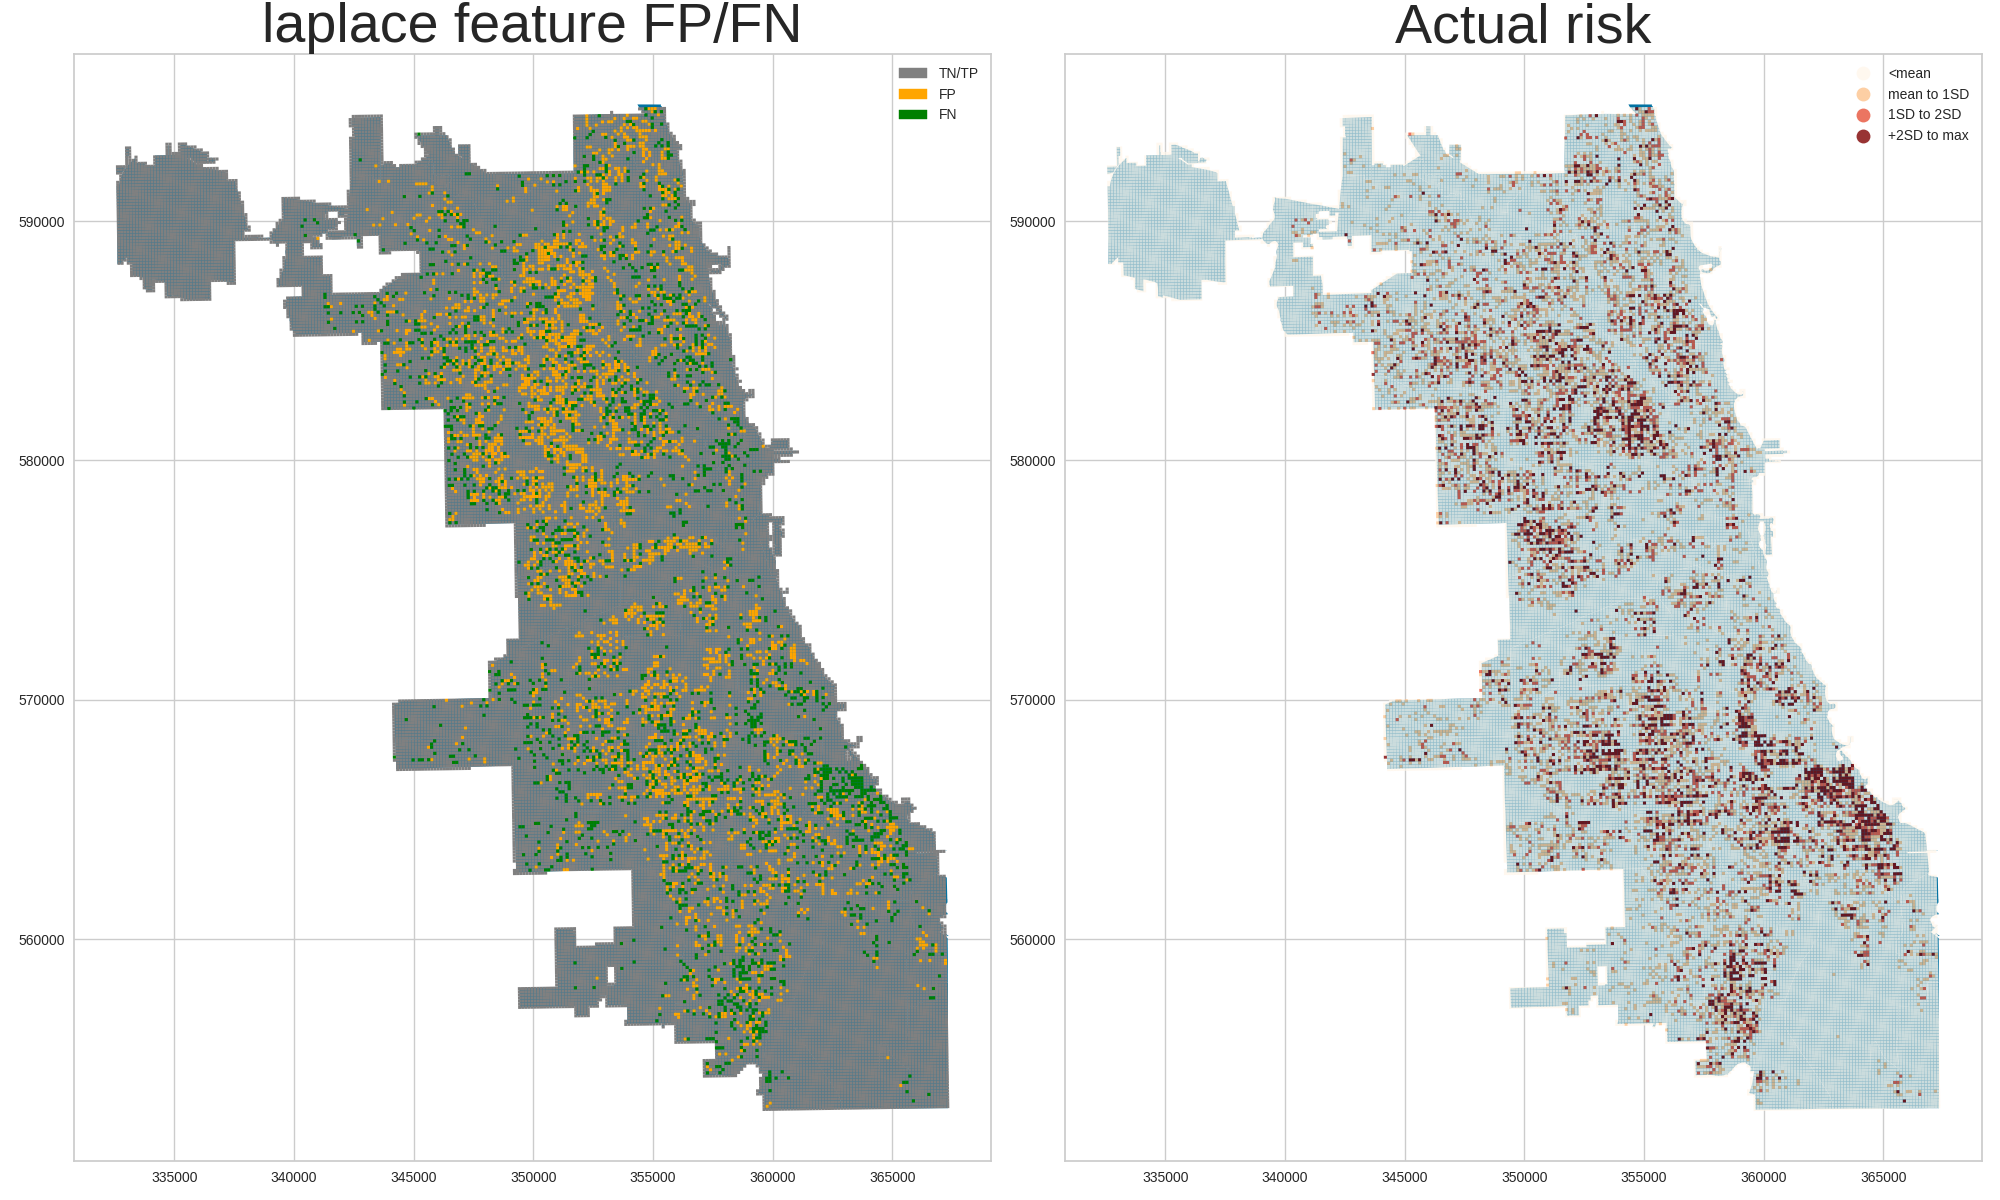
\includegraphics[scale=0.25]{./non-crime-val-figure/laplace_fnp.png}
  \caption{左:ラプラス分布関数特徴量のFPFN 右:実際のリスクマップ}
  \label{fig:nc-val-laplace-fnp}
\end{figure}

\begin{figure}
  \centering % 図を中央寄せにする
  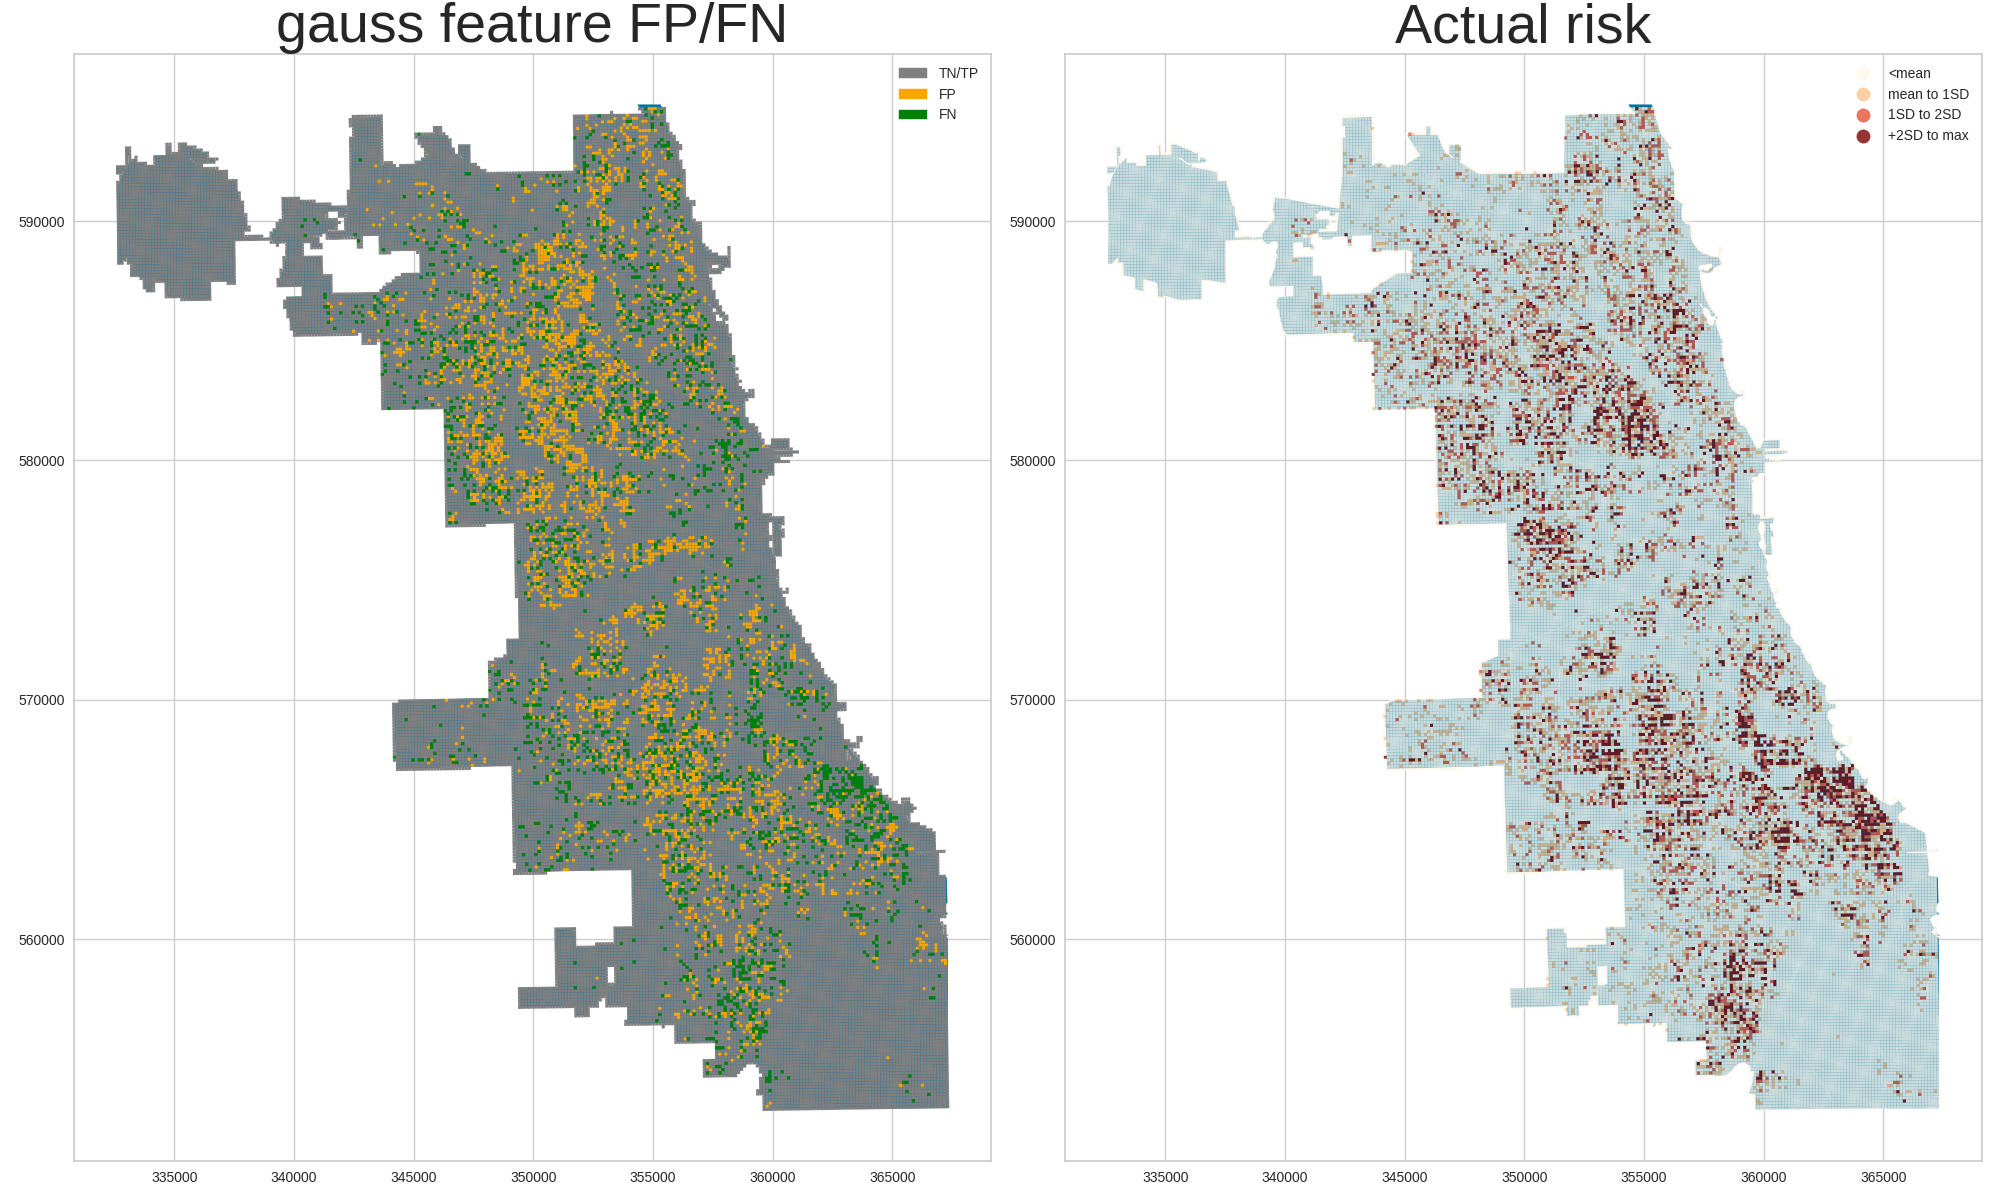
\includegraphics[scale=0.25]{./non-crime-val-figure/gauss_fnp.png}
  \caption{左:ガウス関数特徴量のFPFN 右:実際のリスクマップ}
  \label{fig:nc-val-gauss-fnp}
\end{figure}
%------------------------------------
\section{テスト}
%------------------------------------
%   Chapter 5
\chapter{おわりに}
% \label{chapter_5}
%------------------------------------
これまでに書いた内容を簡潔にまとめる。
ただし,第1章とは異なり,
ここまで論文を読み終えた読者を想定しているため,
これまでに登場した専門用語や事実等を
改めて説明することなく使用してかまわない。
「~を考察した。」ではなく,
「~であることが分かった。」のように
結論を述べる。
今後の課題も書く。


%------------------------------------
%   Acknowledgements
\chapter*{謝辞}
%------------------------------------
\addcontentsline{toc}{chapter}{謝辞}
(研究を遂行するにあたってサポートしてくれた方々へ
謝辞を述べるコーナー。
名前だけでなくどのようなサポートをしてくれたのかも書く。)

(例)
本研究を進めるにあたりご指導頂きました
鈴木一弘先生に感謝いたします。
本論文で主査と副査をして頂きました
\CID{8705}田直樹先生と塩田研一先生に感謝いたします。
日頃の議論を通じて多くの知識や示唆を頂きました
鈴木研究室の皆様に感謝いたします。



%------------------------------------
%   References
%------------------------------------
\bibliography{main} %hoge.bibから拡張子を外した名前
\bibliographystyle{plainnat} %参考文献出力スタイル
%------------------------------------
\appendix
%------------------------------------
\chapter{プログラム}
\label{program}
% \inputminted[breaklines,breakanywhere,linenos,tabsize=4]
% {JavaScript}{discrete_geometry.js}


%------------------------------------
\end{document}
%------------------------------------
